\documentclass[a4paper]{jsbook}
% \usepackage{eulervm}
\usepackage{amsmath,amssymb,ascmac,bm,graphicx,latexsym,mathtools,multirow,okuverb}
\makeindex

\def\[{\left[\!\left[}
\def\]{\right]\!\right]}
\def\({\left(\!\left(}
\def\){\right)\!\right)}

%% Programming Languages

\newcommand{\programminglanguage}[1]{\textsf{#1}}
\newcommand{\clang}{\programminglanguage{C}}
\newcommand{\csharp}{\programminglanguage{C}\texttt{\#}}
\newcommand{\cxx}{\programminglanguage{C}\texttt{++}}
\newcommand{\cxxzerothree}{\cxx\programminglanguage{03}}
\newcommand{\cxxeleven}{\cxx\programminglanguage{11}}
\newcommand{\cxxfourteen}{\cxx\programminglanguage{14}}
\newcommand{\cxxseventeen}{\cxx\programminglanguage{17}}
\newcommand{\haskell}{\programminglanguage{Haskell}}
\newcommand{\java}{\programminglanguage{Java}}
\newcommand{\lisp}{\programminglanguage{LISP}}
\newcommand{\python}{\programminglanguage{Python}}
\newcommand{\ruby}{\programminglanguage{Ruby}}
\newcommand{\scheme}{\programminglanguage{Scheme}}
\newcommand{\swift}{\programminglanguage{Swift}}

%% Leaders and Key Points

\newenvironment{leader}{\begingroup}{\endgroup}
\newenvironment{keypoint}{\begin{screen}}{\end{screen}}
\newenvironment{caution}{\begin{boxnote}\begin{center}注意\end{center}}{\end{boxnote}}

%% Keywords

\newcommand{\keyword}[1]{{\underline{\emph{#1}}}}

%% Inline Codes (like `...` of Markdown doc)

\newcommand{\code}[1]{\texttt{#1}}

%% Code Blocks (like ``` ... ``` of Markdown)

\newenvironment{cxxcode}{\begin{itembox}[r]{\cxx}}{\end{itembox}}
\newenvironment{javacode}{\begin{itembox}[r]{\java}}{\end{itembox}}
\newenvironment{haskellcode}{\begin{itembox}[r]{\haskell}}{\end{itembox}}
\newenvironment{pythoncode}{\begin{itembox}[r]{\python}}{\end{itembox}}
\newenvironment{rubycode}{\begin{itembox}[r]{\ruby}}{\end{itembox}}

%% Math

\newcommand{\mConst}[1]{\text{DO-NOT-USE}}
\newcommand{\mSpecialConst}[1]{\mathrm{#1}} % Internal use
\newcommand{\mTrue}{\mSpecialConst{True}}
\newcommand{\mFalse}{\mSpecialConst{False}}
\newcommand{\mZero}{\O}
\newcommand{\mOne}{\mSpecialConst{I}}
\newcommand{\mVar}[1]{\text{DO-NOT-USE}}
\newcommand{\mSpecialVar}[1]{\mathrm{#1}} % Internal use
\newcommand{\mFirstVar}{\mSpecialVar{first}}
\newcommand{\mRestVar}{\mSpecialVar{rest}}
\newcommand{\mFunc}[1]{\text{DO-NOT-USE}}
\newcommand{\mSpecialSub}[1]{\text{#1}}
\newcommand{\mLeft}{\mSpecialSub{left}}
\newcommand{\mRight}{\mSpecialSub{right}}
\newcommand{\mSet}[1]{\mathbf{#1}}
\newcommand{\mSpecialSet}[1]{\mathbb{#1}} % Internal use
\newcommand{\mRSet}{\mSpecialSet{R}}
\newcommand{\mQSet}{\mSpecialSet{Q}}
\newcommand{\mZSet}{\mSpecialSet{Z}}
\newcommand{\mBSet}{\mSpecialSet{B}}
\newcommand{\mTypeParameter}[1]{\mathbf{#1}}
\newcommand{\mType}[1]{\mathbf{#1}}
\newcommand{\mBoolType}{\mType{Bool}}
\newcommand{\mCharType}{\mType{Char}}
\newcommand{\mIntType}{\mType{Int}}
\newcommand{\mFloatType}{\mType{Float}}
\newcommand{\mListType}[1]{[\mType{#1}]}
\newcommand{\mMaybeType}[1]{\[\mType{#1}\]}
\newcommand{\mFunctor}[1]{\textit{\textbf{#1}}}
\newcommand{\mSpecialFunctor}[1]{\mathcal{#1}} % Internal use
\newcommand{\mTypeConstructor}[1]{\mathit{#1}} % Internal use
\newcommand{\mSpecialTypeClass}[1]{\mathfrak{#1}} % Inetrnal use
\newcommand{\mEqTypeClass}{\mSpecialTypeClass{Eq}}
\newcommand{\mOrdTypeClass}{\mSpecialTypeClass{Ord}}
\newcommand{\mNumTypeClass}{\mSpecialTypeClass{Num}}
\newcommand{\mRealTypeClass}{\mSpecialTypeClass{Real}}
\newcommand{\mEnumTypeClass}{\mSpecialTypeClass{Enum}}
\newcommand{\mIntegralTypeClass}{\mSpecialTypeClass{Integral}}
\newcommand{\mMonoidTypeClass}{\mSpecialTypeClass{Monoid}}
\newcommand{\mFunctorTypeClass}{\mSpecialTypeClass{Functor}}
\newcommand{\mEmptyList}{{[\,]}}
\newcommand{\mNothing}{\emptyset}
\newcommand{\mPureNothing}{\varnothing}
\newcommand{\mKeyword}[1]{\mathsf{#1}}
\newcommand{\mIfKeyword}{\mKeyword{if}}
\newcommand{\mOtherwiseKeyword}{\mKeyword{otherwise}}
\newcommand{\mThenKeyword}{\mKeyword{then}}
\newcommand{\mElseKeyword}{\mKeyword{else}}
\newcommand{\mCaseKeyword}{\mKeyword{case}}
\newcommand{\mOfKeyword}{\mKeyword{of}}
\newcommand{\mLetKeyword}{\mKeyword{let}}
\newcommand{\mInKeyword}{\mKeyword{in}}
\newcommand{\mWhereKeyword}{\mKeyword{where}}
\newcommand{\mListWith}[1]{\left[#1\right]}
\newcommand{\mSetWith}[1]{\left\{#1\right\}}
\newcommand{\mTupleWith}[1]{\left(#1\right)}
\newcommand{\mMaybeWith}[1]{\[#1\]}
\newcommand{\mPureWith}[1]{\langle\!\langle#1\rangle\!\rangle}
\newcommand{\mUnitWith}[1]{\langle#1\rangle}
\newcommand{\mList}[1]{{#1}^\mathrm{\star}}
\newcommand{\mMaybe}[1]{{#1}^\text{?}}
% \newcommand{\mContainerVar}[1]{\Check{#1}}
\newcommand{\mAnonParameter}{\lozenge}
\newcommand{\mAnyParameter}{\_}
\newcommand{\mMonadFunc}[1]{#1}%{{\boldsymbol#1}}

\newcommand{\mGuard}[1]{\mathop{\mid_{#1}}}

\DeclareMathOperator{\mIfFunc}{if}
\DeclareMathOperator{\mLambda}{\backslash}
\DeclareMathOperator{\mLambdaArrow}{\rightarrow}
\DeclareMathOperator{\mIn}{{:\!:}}
\DeclareMathOperator{\mSum}{sum}
\DeclareMathOperator{\mMapsTo}{\mapsto}
\DeclareMathOperator{\mBinOp}{\bigstar}
\DeclareMathOperator{\mComp}{\cdot}
\DeclareMathOperator{\mApply}{\$}
\DeclareMathOperator{\mApplyRight}{\rightsquigarrow}
\DeclareMathOperator{\mFlow}{\leadsto}
\DeclareMathOperator*{\mFoldLeft}{\bigcup}
\DeclareMathOperator*{\mFoldRight}{\bigsqcup}
\DeclareMathOperator{\mCons}{:}
\DeclareMathOperator{\mConcat}{\flat}
\DeclareMathOperator{\mAppend}{\oplus}
\DeclareMathOperator{\mMap}{\bullet}
\DeclareMathOperator{\mMapList}{\odot}
\DeclareMathOperator{\mMapMaybe}{\boxdot}
\DeclareMathOperator{\mAMap}{\times}
\DeclareMathOperator{\mAMapList}{\otimes}
\DeclareMathOperator{\mAMapMaybe}{\boxtimes}
\DeclareMathOperator{\mApplicativeApply}{\S}
\DeclareMathOperator{\mApplicativeMap}{\times}
\DeclareMathOperator{\mApplicativeMapList}{\otimes}
\DeclareMathOperator{\mApplicativeMapMaybe}{\boxtimes}
\DeclareMathOperator{\mBindList}{\clubsuit}%{\leftleftarrows}
\DeclareMathOperator{\mBindListRight}{\rightrightarrows}
\DeclareMathOperator{\mBindMaybe}{\spadesuit}%{\dashleftarrow}
\DeclareMathOperator{\mBindMaybeRight}{\dashrightarrow}
\DeclareMathOperator{\mBind}{\heartsuit}%{\twoheadleftarrow}
\DeclareMathOperator{\mBindRight}{\twoheadrightarrow}
% \DeclareMathOperator{\mBindLeft}{\ooalign{$\longleftarrow$\crcr\hss$\heartsuit$\hss}}
% \DeclareMathOperator{\mBindRight}{\ooalign{$\longrightarrow$\crcr\hss$\heartsuit$\hss}}
\DeclareMathOperator{\mLogicalAnd}{\wedge}
\DeclareMathOperator{\mLogicalOr}{\vee}
\DeclareMathOperator{\mFrom}{\in}
\DeclareMathOperator{\mPred}{pred}
\DeclareMathOperator{\mSucc}{succ}
\DeclareMathOperator{\mHead}{head}
\DeclareMathOperator{\mTail}{tail}
\DeclareMathOperator{\mListTypeConstructor}{\mTypeConstructor{List}}
\DeclareMathOperator{\mMaybeTypeConstructor}{\mTypeConstructor{Maybe}}
\DeclareMathOperator{\mIFunctor}{\mSpecialFunctor{I}}
\DeclareMathOperator{\mListFunctor}{\mFunctor{List}}
\DeclareMathOperator{\mMaybeFunctor}{\mFunctor{Maybe}}
\DeclareMathOperator{\mListProjection}{\xmapsto{\;\mListFunctor\;}}
\DeclareMathOperator{\mMaybeProjection}{\xmapsto{\;\mMaybeFunctor\;}}
\DeclareMathOperator{\mIf}{\mIfKeyword}
\DeclareMathOperator{\mOtherwise}{\mOtherwiseKeyword}
\DeclareMathOperator{\mThen}{\mThenKeyword}
\DeclareMathOperator{\mElse}{\mElseKeyword}
\DeclareMathOperator{\mWhere}{\mWhereKeyword}
\DeclareMathOperator{\mCase}{\mCaseKeyword} % Internal use
\DeclareMathOperator{\mOf}{\mOfKeyword} % Internal use
\DeclareMathOperator{\mLet}{\mLetKeyword} % Internal use
\DeclareMathOperator{\mInKW}{\mInKeyword} % Internal use

\newcommand{\mCaseOf}[1]{\mCase{#1}\mOf}
\newcommand{\mLetIn}[2]{\mLet{#1}\mInKW{#2}}
\newcommand{\mIfThenElse}[3]{\mIf{#1}\mThen{#2}\mElse{#3}}
\newcommand{\mLambdaExp}[2]{\mLambda{#1}\mLambdaArrow{#2}}
\newcommand{\mProjection}[2]{#1\mMapsTo#2}


%% Math Pretty Printers

\newcommand{\mConnst}[1]{\mathrm{#1}} % Use capital letter
\newcommand{\mathSub}[1]{\textrm{#1}}

\newcommand{\mathSet}[1]{\mathbf{#1}} % Use capital letter
\newcommand{\mathSpecialSet}[1]{\mathbb{#1}} % Use capital letter
\newcommand{\mathTypeParameter}[1]{\mathbf{#1}}
\newcommand{\mathTypeName}[1]{\mathTypeParameter{#1}}
\newcommand{\mathTypeParameterClass}[1]{\mathbf{\emph{#1}}}

\newcommand{\mathFunctor}[1]{\textsl{#1}} % Use capital letter
\newcommand{\mathSpecialFunctor}[1]{\mathcal{#1}} % Use capital letter
\newcommand{\mathTypeConstructor}[1]{\mathit{#1}} % Use capital letter
\newcommand{\mathTypeClass}[1]{\textbf{\emph{#1}}} % Use capital letter

%% Hats for Variables

\newcommand{\mathListVar}[1]{\Bar{#1}}
\newcommand{\mathMaybeVar}[1]{\Tilde{#1}}
\newcommand{\mathFunctionVar}[1]{\Hat{#1}}
\newcommand{\mathContainerVar}[1]{\Check{#1}}
\newcommand{\mathVectorVar}[1]{\vec{#1}}

%% Parenthesis for Variables

\newcommand{\mathListWith}[1]{\left[#1\right]}
\newcommand{\mathSetWith}[1]{\left\{#1\right\}}
\newcommand{\mathTupleWith}[1]{\left(#1\right)}
\newcommand{\mathMaybeWith}[1]{\[#1\]}
\newcommand{\mathPureWith}[1]{\left\langle#1\right\rangle}
\newcommand{\mathUnitWith}[1]{\left\langle\!\left\langle#1\right\rangle\!\right\rangle}

%% Parenthesis for Types

\newcommand{\mathListType}[1]{\mathListWith{\mathTypeParameter{#1}}}
\newcommand{\mathMaybeType}[1]{\mathMaybeWith{\mathTypeParameter{#1}}}
\newcommand{\mathPureType}[1]{\mathPureWith{\mathTypeParameter{#1}}}
\newcommand{\mathUnitType}[1]{\mathUnitWith{\mathTypeParameter{#1}}}

%% Guard

\newcommand{\mathGuard}[1]{\mathop{\mid_{#1}}}

%% Type Constructors and Functors

\DeclareMathOperator{\mathList}{\mathTypeConstructor{List}}
\DeclareMathOperator{\mathMaybe}{\mathTypeConstructor{Maybe}}
\DeclareMathOperator{\mathListFunctor}{\mathFunctor{List}}
\DeclareMathOperator{\mathMaybeFunctor}{\mathFunctor{Maybe}}

%% True and Fasle, Identity, Empty, Nothing

\newcommand{\mathTrue}{\mConst{T}}
\newcommand{\mathFalse}{\mConst{F}}

\newcommand{\mathId}{\O}

\newcommand{\mathEmptyList}{{[\,]}}
\newcommand{\mathNothing}{\emptyset}
\newcommand{\mathPureNothing}{\varnothing}

%% Special Parameters

\newcommand{\mathAnonymousParameter}{\lozenge}
\newcommand{\mathAny}{\_}
\newcommand{\mathSomething}{\square}  % DO NOT USE

%% Left and Right

\newcommand{\mathLeft}{\mathSub{left}}
\newcommand{\mathRight}{\mathSub{right}}

%% Special Unary Functions and Operators

\DeclareMathOperator{\mathPred}{pred}
\DeclareMathOperator{\mathSucc}{succ}
\DeclareMathOperator{\mathAnyUnaryOperator}{\star}
\DeclareMathOperator{\mathInverse}{\sharp}  % USED?
\DeclareMathOperator{\mathLambda}{\backslash}
\DeclareMathOperator{\mathConcat}{\flat}
\DeclareMathOperator*{\mathFold}{\bigcup}
\DeclareMathOperator*{\mathFoldRight}{\bigsqcup}

\DeclareMathOperator{\mathHead}{head}
\DeclareMathOperator{\mathTail}{tail}
\DeclareMathOperator{\mathFactorial}{fact}
\DeclareMathOperator{\mathIfFunc}{if}

\DeclareMathOperator{\mathMain}{main}

%% Special Binary Operators

\newcommand{\mathAnyBinaryOperator}{\mathbin{\bigstar}}
\newcommand{\mathAnd}{\mathbin{\wedge}}
\newcommand{\mathAppend}{\oplus}
\newcommand{\mathApplicativeApply}{\mathbin{\S}}
\newcommand{\mathApplicativeGeneralMap}{\mathbin{\times}}
\newcommand{\mathApplicativeMap}{\mathbin{\otimes}}
\newcommand{\mathApplicativeMaybeMap}{\mathbin{\boxtimes}}
\newcommand{\mathApply}{\mathbin{\$}}
\newcommand{\mathBind}{\mathbin{\ooalign{$\longleftarrow$\crcr\hss$\heartsuit$\hss}}}
\newcommand{\mathBindRight}{\mathbin{\ooalign{$\longrightarrow$\crcr\hss$\heartsuit$\hss}}}
\newcommand{\mathCompose}{\mathbin{\bullet}}
\newcommand{\mathGeneralMap}{\mathbin{\cdot}}
\newcommand{\mathFrom}{\mathbin{\in}}
\newcommand{\mathIn}{\mathrel{::}}
\newcommand{\mathMap}{\mathbin{\odot}}
\newcommand{\mathMaybeAppend}{\mathbin{\boxplus}}
\newcommand{\mathMaybeMap}{\mathbin{\boxdot}}
\newcommand{\mathOr}{\mathbin{\vee}}
\newcommand{\mathSetTimes}{\mathbin{\circledast}}

%% Special Arrow Operators

\newcommand{\mathLambdaArrow}{\rightarrow}
\newcommand{\mathMapsTo}{\mapsto}

%% Keywords

\newcommand{\mathKeyword}[1]{\operatorname{\textsf{#1}}}

\newcommand{\mathIf}{\mathKeyword{if}}
\newcommand{\mathThen}{\mathKeyword{then}}
\newcommand{\mathElse}{\mathKeyword{else}}
\newcommand{\mathOtherwise}{\mathKeyword{otherwise}}

\newcommand{\mathCaseCase}{\mathKeyword{case}}
\newcommand{\mathCaseOf}{\mathKeyword{of}}

\newcommand{\mathLetLet}{\mathKeyword{let}}
\newcommand{\mathLetIn}{\mathKeyword{in}}
\newcommand{\mathWhere}{\mathKeyword{where}}

%% First and Rest

\newcommand{\mathVarKeyword}[1]{\operatorname{\mathrm{#1}}}

\newcommand{\mFirstVar}{\mathVarKeyword{first}}
\newcommand{\mathRest}{\mathVarKeyword{rest}}

%% Utilities

\newcommand{\mathCase}[2]{\mathCaseCase#1\mathCaseOf#2}
\newcommand{\mathCategoryShort}[2]{(#1,#2)}
\newcommand{\mathLambdaExpression}[2]{\mathLambda#1\mathLambdaArrow#2}
\newcommand{\mathLet}[2]{\mathLetLet#1\mathLetIn#2}
\newcommand{\mathMorph}[2]{#1\mathMapsTo#2}

\newcommand{\mathMonoid}[3]{(#1,#2,#3)}
\newcommand{\mathMorphII}[3]{#1\mathMapsTo#2\mathMapsTo#3}
\newcommand{\mathMorphIIWithParenthesis}[3]{#1\mathMapsTo(#2\mathMapsTo#3)}

\newcommand{\mathCategory}[4]{(#1,#2,#3,#4)}
\newcommand{\mathGroup}[4]{(#1,#2,#3,#4)}
\newcommand{\mathMorphIII}[4]{#1\mathMapsTo#2\mathMapsTo#3\mathMapsTo#4}

\newcommand{\mathField}[7]{(#1,#2,#3,#4,#5,#6,#7)}

%% Haskell Operators

\DeclareMathOperator{\hsklConcat}{{DO NOT USE}--\flat}
\DeclareMathOperator{\hsklFmap}{{DO NOT USE}--\cdot}
\DeclareMathOperator{\hsklHead}{{DO NOT USE}--head}
\DeclareMathOperator{\hsklMap}{{DO NOT USE}--\odot}
\DeclareMathOperator{\hsklMaybeAppend}{{DO NOT USE}--\boxplus}
\DeclareMathOperator{\hsklMaybeMap}{{DO NOT USE}--\boxdot}
\DeclareMathOperator{\hsklMonadMap}{{DO NOT USE}--\heartsuit}
\DeclareMathOperator{\hsklOf}{{DO NOT USE}--::}
\DeclareMathOperator{\hsklTail}{{DO NOT USE}--tail}

%% Haskell Symbols


%% Haskell Types and Type Classes

\newcommand{\hsklApplicative}{{DO NOT USE}--\mathTypeParameterClass{Applicative}}
\newcommand{\hsklBool}{{DO NOT USE}--\mathTypeParameter{Bool}}
\newcommand{\hsklChar}{{DO NOT USE}--\mathTypeParameter{Char}}

\newcommand{\hsklIntegral}{{DO NOT USE}--\mathTypeParameterClass{Integral}}
\newcommand{\hsklFloat}{{DO NOT USE}--\mathTypeParameter{Float}}
\newcommand{\hsklFunctor}{{DO NOT USE}--\mathTypeParameterClass{Functor}}
\newcommand{\hsklMonad}{{DO NOT USE}--\mathTypeParameterClass{Monad}}
\newcommand{\hsklMonadplus}{{DO NOT USE}--\mathTypeParameterClass{Monadplus}}

%% Haskell Value Constructors

\newcommand{\hsklJust}[1]{{DO NOT USE}--\[#1\]}
\newcommand{\hsklListType}[1]{{DO NOT USE}--[#1]}
\newcommand{\hsklMaybeType}[1]{{DO NOT USE}--\[#1\]}
\newcommand{\hsklPure}[1]{{DO NOT USE}--\langle#1\rangle_\textsf{pure}}
\newcommand{\hsklUnit}[1]{{DO NOT USE}--\langle#1\rangle_\textsf{unit}}

%% Haskell Type Constructor

\newcommand{\hsklTypeParameterConstruct}[2]{{DO NOT USE}--#1\,#2}

%% Haskell Decorations

\newcommand{\hsklFunction}[1]{{DO NOT USE}--\Hat{#1}}
\newcommand{\hsklMaybe}[1]{{DO NOT USE}--\Tilde{#1}}
\newcommand{\hsklMaybeW}[1]{{DO NOT USE}--\widetilde{#1}}


\title{\haskell (仮)}
\author{金谷一朗}

\begin{document}
\setlength{\baselineskip}{17pt}
\maketitle
\tableofcontents

\begin{table*}
\caption{凡例}
\begin{center}
\begin{tabular}{||c|c|c||}
\hline
種類&字体・表記法&例\\
\hline\hline
定数&イタリック,大文字&$A,B,C$\\
有名な定数&ローマン,大文字&$\mTrue,\mFalse$\\
\hline
変数&イタリック,小文字&$m,n,x,y,z$\\
有名な変数&ローマン,小文字&$\mFirstVar,\mRestVar$\\
リスト変数&肩に星印をつける&$\mList{x}$\\
Maybe変数&肩に?をつける&$\mMaybe{m}$\\
% 一般コンテナ変数&イタリック,ギリシア文字&$\alpha,\beta,\omega$\\
\hline
関数&イタリック,小文字&$a,b,f,g,h$\\
有名な関数&ローマン,小文字&$\sin,\cos$\\
リスト関数&肩に星印をつける&$\mList{f}$\\
Maybe関数&肩に?をつける&$\mMaybe{a}$\\
% 一般コンテナ関数&イタリック,ギリシア文字&$\phi,\psi$\\
モナドを返す関数&ギリシア文字&$\mMonadFunc{\mu}$\\
\hline
添字&ローマン,小文字&$x_\mLeft,x_\mRight$\\
\hline
集合&ボールドローマン,大文字&$\mSet{A},\mSet{B},\mSet{C}$\\
有名な集合&ブラックボード,大文字&$\mBSet,\mZSet,\mRSet$\\
単位元&ローマンに斜線,大文字&$\mZero$\\
\hline
型パラメタ&ボールドローマン,小文字&$\mTypeParameter{a},\mTypeParameter{b},\mTypeParameter{c}$\\
型&ボールドローマン,大文字&$\mBoolType,\mIntType,\mFloatType$\\
型クラス&フラクチュール,大文字&$\mEqTypeClass,\mOrdTypeClass,\mNumTypeClass$\\
\hline
型コンストラクタ&イタリック,大文字&$\mListTypeConstructor$, $\mMaybeTypeConstructor$\\
関手&ボールドイタリック,大文字&$\mFunctor{List},\mFunctor{Maybe}$\\
有名な関手&カリグラフィ,大文字&$\mIFunctor$\\
\hline
キーワード&サンセリフ,小文字&$\mIf,\mOtherwise$\\
% リストの構造&サンセリフ,大文字&$\mathFirst$, $\mathRest$\\
\hline
リスト&ブラケットで包む&$\mListWith{x,y,z}$\\
集合&ブレースで包む&$\mSetWith{x,y,z}$\\
タプル&丸括弧で包む&$\mTupleWith{x,y,z}$\\
\hline
\end{tabular}
\end{center}
\end{table*}

\begin{table*}[p]
\caption{記号一覧}
\begin{center}
\begin{tabular}{||c|c|c||}
\hline
記号&意味&最初に登場するページ\\
\hline\hline
$\mLambda, \mLambdaArrow$&ラムダ式&\\
$\mAnonParameter$&無名パラメタ&\\
\hline
$\mIn$&集合の元&\\
$\in$&集合の元&\\
$\mMapsTo$&写像&\\\hline
$\mBinOp$&任意の二項演算子&\\
$\mComp$&関数合成&\\
$\mApply$&関数適用&\\
$\mApplicativeApply$&アプリカティブ関数適用&\\
$\mApplyRight$&関数の右適用&\\\hline
$\mFoldLeft$&左畳み込み&\\
$\mFoldRight$&右畳み込み&\\
\hline
$\mCons$&結合 (cons)&\\
$\mConcat$&平坦化 (concat)&\\
$\mAppend$&リスト結合 (append)&\\
% $\mathMaybeAppend$&Maybe結合&\\
\hline
$\mEmptyList$&空リスト&\\
$\mNothing$&空Maybe(ナッシング)&\\
$\mPureNothing$&空&\\\hline
$\mListWith{x}$&リスト値コンストラクタ&\\
$\mMaybeWith{x}$&Maybe値コンストラクタ&\\
$\mPureWith{x}$&ピュア演算子&\\
$\mUnitWith{x}$&ユニット演算子&\\
\hline
$\mMap$&一般マップ&\\
$\mMapList$&リストのマップ&\\
$\mMapMaybe$&Maybeのマップ&\\
\hline
$\mAMap$&一般アプリカティブマップ&\\
$\mAMapList$&リストのアプリカティブマップ&\\
$\mAMapMaybe$&Maybeのアプリカティブマップ&\\
\hline
$\mBindList$&リストのバインド演算子&\\
$\mBindMaybe$&Maybeの左バインド演算子&\\
$\mBind$&モナドのバインド演算子&\\
\hline
\end{tabular}
\end{center}
\end{table*}

\part{代数的構造とプログラミング}

\chapter{はじめに}

\begin{leader}
本書はプログラミング言語\haskell の入門書である.
\end{leader}

\section{\haskell という森*}

これからのプログラマにとって\haskell を無視することはできない.\haskell の「欠点をあげつらうことも,攻撃することもできるが,無視することだけはできない」のだ.それは\haskell がプログラミングの本質に深く関わっているからである.

\haskell というプログラミング言語を知ろうとすると,従来のプログラミング言語の知識が邪魔をする.モダンで,人気があって,\haskell から影響を受けた言語,例えば\ruby や\swift の知識さえ,\haskell を学ぶ障害になり得る.ではどのようにして\haskell の深みに到達すればいいのだろうか.

その答えは,一見遠回りに見えるが,一度抽象数学の高みに登ることである.

と言っても,あわてる必要はない.

近代的なプログラミング言語を知っていれば,すでにある程度抽象数学に足を踏み入れているからである.そこで,本書では近代的なプログラマを対象に,プログラミング言語を登山口に抽象数学の山を登り,その高みから\haskell という森を見下ろすことにする.

%% REWRITE %%

さて,登山口にどのプログラミング言語を選ぶのが適当であろうか.IEEE Spectrum の ``The 2015 Top Ten Programming Languages'' という記事によると「ビッグ5」として \java, \clang, \cxx, \python, \csharp\ が挙げられている.このうち\clang は「多くのプログラマが読める」以外にメリットが無く,その唯一のメリットさえ最近は怪しくなっているため,登山口候補から外す.残るは \java, \cxx, \csharp\ グループと\python ということになるが,シンプルであり,かつ\haskell と対極にある言語である\python(バージョン3)を登山口に選ぶことにした.

本書では\python コードはこのように登場する.
\begin{pythoncode}
\begin{verbatim}
print "Hello, world."
\end{verbatim}
\end{pythoncode}
本書に示すコードは擬似コードではなく,すべて実行可能な本物のコードである.

ところで,一部の章でどうしても型に触れないといけない部分がある.\python は動的型付け言語であり,型の説明には不適切であるため,この部分だけ理解の助けとして\cxxfourteen によるコードを例示した.この部分はコードを読まなくても先に進める.\java ではなく\cxx を採用したのはmacOSでも簡単に試せるようにである.型システムに関する限り\cxx よりも\java のほうが簡潔に記述できるが,致し方無い.

\section{関数型プログラミング}

ところで,プログラマはなぜ\haskell を習得しなければならないのだろう.それは\haskell と\keyword{関数型プログラミング}の間に密接な関係があるからである.

関数型プログラミングとはプログラミングにおける一種のスローガンのようなもので,どの言語を用いたから関数型でどの言語を用いたから関数型ではない,というものではない.しかし,関数型プログラミングを強くサポートする言語と,そうでない言語とがある.ここら辺の事情はオブジェクト指向プログラミングとプログラミング言語の関係と似ている.\haskell は関数型プログラミングを強くサポートし,\python はほとんどサポートしない.

関数型プログラミングの特徴を一言で言えば,プログラム中の\keyword{破壊的代入}を禁止することである.変数 $x$ に $1$ という数値が一度代入されたら,変数 $x$ の値をプログラム中に書き換える,すなわち破壊的代入をすることはできない.この結果,変数の値はプログラムのどこでも,どの時点で読み出しても同じであることが保証される.これを変数の\keyword{参照透過性}と呼ぶ.

プログラム全体に参照透過性があると,そのプログラムはブロックに分割しやすく,各々のブロックは再利用しやすい.またプログラムのどの断片から読み始めても,全体の構造を見失いにくい.これが関数型プログラミングとそれを強くサポートする\haskell を習得する理由である.

% \section{数学とプログラミングの関係*}

% 数学とプログラミングの関係について述べておこう.ある方程式を解くためにコンピュータによって数値シミュレーションを行うとか,非常に複雑な微分を機械的に行うとか,プログラミングによって数学をサポートすることは計算機科学の主たる分野の一つであるが,ここではもっと根源的な話をする.

% 数学者もプログラマも\keyword{関数}をよく使う.数学者が使う関数とは,引数がいくつかあって,その結果決まる戻り値があるようなものだ.一方でプログラマが使う関数というのは,引数と戻り値はだいたい同じとして,中身に条件分岐があったり,ループがあったり,外部変数を書き換えたり,入出力をしたりする.

% どちらも同じ関数,なぜこうもイメージが違うのだろうか.

% もし,我々が関数型プログラミングの原則を忠実に守り,プログラム中のいかなる破壊的代入をも禁止するとすると,両者の関数は全く同じ性格になる.条件分岐もループも,それどころか定数さえ,\keyword{ラムダ式}という式だけで書けるようになる.あらゆるプログラムが,最終的には単一のラムダ式で書ける.

% ラムダ式は単純で,十分に数学的に定式化できるものだ.

\section{\haskell コンパイラの準備*}

\haskell コンパイラの中で最もよく使われているものは Glasgow's Haskell Compiler (GHC) である.本書に登場する\haskell コードもすべてGHCでテストをしている.

GHCは公式サイト\cite{haskellplatform}からダウンロード可能であるが,GNU/Linuxシステム(以下Linux),macOSはそれぞれのパッケージマネージャからインストールすることを勧める.インストール方法は以下の参考文献にアクセスしてもらいたい.
\begin{description}
\item[Linux] パッケージマネージャからghciをインストールする.Debian系ならAPT,Red Hat系ならYumを使うのが一般的であろう.文献\cite{linux}を参考にしてもらいたい.
\item[macOS] 文献\cite{osx}にHomebrewのインストール方法が書かれているので,Homebrewのインストールまでしておき,ターミナルで
\begin{verbatim}
$ brew install ghci
\end{verbatim} %$
とする.(本書執筆時点でHaskell Stackという新しいパッケージングシステムが登場してきている.
将来的にはGHC本体もHaskell Stackからインストールすることが望ましくなるだろう.Haskell Stackを用いたGHCのインストールはmacOSではHomebrewを用いて
\begin{verbatim}
$ brew install haskell-stack
$ stack install ghc
\end{verbatim} %$ %$
とすれば良い.本書はひとまずGHCを直接インストールすることを前提に進める.)
\item[Windows 10] GHC公式サイト\cite{haskellplatform}からパッケージをインストールする.
\end{description}

\section{余計な話:本書の構成*}

ところで,各章の終りにはこのような「余計な話」の節を設けている.余計な話には,本書を読み進めるに当たって本質的ではない話を詰め込んでいる.ではなぜ書くかというと,これは筆者が頭を整理するために書くのである.なので,筆者が何を思って本書を執筆していたかを知りたいときが万が一来れば,目を通してもらいたい.

最初の余計な話は本書の構成である.

そもそも本の構成など,目次を見ればわかることであるが,執筆時点では目次がまだない.そこで,筆者がときどきこの節を読み返し,全体の構成を確認しているのである.

本書は3部構成になっている.第I部はプログラミング言語から抽象数学への登山である.第II部は抽象数学の山頂から\haskell の森へ下っていく道である.第III部はこれまで歩いた道全体を俯瞰する.

第I部は対応する\haskell のコードを脚注に記載している.脚注部分は\haskell を一通り覚えた後で読み返してもらいたい.\footnote{\haskell のコードは \code{x = 1} のようにタイプライタ体で書く.}

\chapter{カリー風な書き方}
\begin{leader}
本書では一般の数学書やプログラミングの教科書からは少し異なった記法を用いる.ある概念が発明されてからずっと後になって正しい記法が見つかり,それがきっかけとなって正しく理解されるという現象は歴史上よくあることである.本書でも様々な新しい記号,記法を導入するが,この章では\haskell に近い記法から始めることにする.
\end{leader}

\section{関数}

数学やプログラミミング言語には書き方に一定の決まりがある.この章ではまず「カリー風の」数式記述方式を見てみることにする.「カリー風」というのは,数学者ハスケル・カリーから名前を借りた言い方で,筆者が勝手に命名したものだ.

カリー風の書き方は数学の教科書やプログラミングの教科書で見かけるものとは若干違うが,圧倒的にシンプルで\haskell との親和性も高く,慣れてくると非常に読みやすいものなので,本書でも全面的に採用する.

まずは\keyword{関数}から見ていくことにしよう.\python や一般的な数学書では引数 $x$ をとる関数 $f$ を
\begin{pythoncode}
\begin{verbatim}
f(x)
\end{verbatim}
\end{pythoncode}
と書くが,括弧は冗長なので今後は
\begin{equation}
fx
\end{equation}
と書くことにする.\footnote{\haskell では関数 \code{f} に引数 \code{x} を適用させることを  \code{f x} と書く.}

% 本書では\python のコード片は上述のように囲みにいれることにする.

関数 $f$ に引数 $x$を「食わせる」ことを\keyword{関数適用}と呼ぶ.もし $fx$ と書いてあったら,それは $f$ と $x$ の積,つまり $f*x$ ではなく,従来の $f(x)$ すなわち関数 $f$ に引数 $x$ を与えているものと解釈する.高校生向けの数学書でも $\sin x$ のように三角関数に限ってはカリー風に書くことになっているので,まるで馴染みがないということもないだろう.なお,関数はいつも引数の左側に書くことにする.これを「関数が\keyword{左から作用する}」と言う.

複数引数をとる関数を\python では
\begin{pythoncode}
\begin{verbatim}
g(x,y)
\end{verbatim}
\end{pythoncode}
と書くが,これも括弧が冗長なので今後は $gxy$ と書く.この場合式 $gxy$ は左を優先して結合する.つまり
\begin{equation}
gxy=(gx)y
\end{equation}
である.これは引数 $y$ に関数 $(gx)$ が作用していると解釈する.関数 $(gx)$ は引数 $x$ に関数 $g$ を作用させて作った関数である.引数に「飢えた」関数 $(gx)$ を\keyword{部分適用}された関数と呼ぶ.

このように式の左側を優先的に演算していくことを\keyword{左結合}と呼ぶ.関数適用は左結合である.

関数はいつも適用する変数の左側に置く.このように左に置く関数のことを数学者は\keyword{左作用素}と呼ぶ.

\section{ラムダ式}

引数 $x$ をとり値 $1+x$ を返す\keyword{ラムダ式}を\python では
\begin{pythoncode}
\begin{verbatim}
lambda x: 1+x
\end{verbatim}
\end{pythoncode}
と書くが,我々はより簡潔に
\begin{equation}
\mLambdaExp{x}{1+x}
\end{equation}
と書くことにする.この式はラムダ式を発明したチャーチのオリジナルの論文の記法であれば $\Hat{x}\,.\,1+x$ と書かれたところであり,現在でも多くの書物で $\lambda x\,.\,1+x$ と記述されるところである.しかし我々はすべてのギリシア文字を変数名のために予約しておきたいのと,ピリオド記号 $(.)$ が今後登場する二項演算子 $\cdot$ と紛らわしいため,上述の記法を用いる.\footnote{\haskell ではラムダ式 $\mLambdaExp{x}{1+x}$ を \code{\textbackslash x -> 1+x} と書く.}

ラムダ式は関数である.ラムダ式を適用するには,ラムダ式を括弧で包む必要がある.例を挙げる.
\begin{equation}
(\mLambdaExp{x}{1+x})2
\end{equation}
この式は結果として $3$ を返す.

複数引数をとるラムダ式は例えば
\begin{equation}
\mLambdaExp{xy}{x+y}
\end{equation}
のように引数を並べて書く.

本書では新たに,次のラムダ式記法も導入する.式中に記号 $\mAnonParameter$ が現れた場合,その式全体がラムダ式であるとみなす.記号 $\mAnonParameter$ の部分には引数が入る.第 $n$ 番目の $\mAnonParameter$ には第 $n$ 番目の引数が入る.例えばラムダ式 $\mLambdaExp{xy}{x+y}$ は
\begin{equation}
\mAnonParameter+\mAnonParameter
\end{equation}
と書いても良い.式を左から読んで1番目の $\mAnonParameter$ が元々の $x$ すなわち第1引数を,2番目の $\mAnonParameter$ が元々の $y$ すなわち第2引数を意味する.この省略記法はプログラミング言語\scheme における\code{cut}プロシジャに由来する.\footnote{この記法は\haskell にはない.}

\section{関数定義}

関数 $f$ を $fx=(\sin x)/x$ と定義したいときに,\python では
\begin{pythoncode}
\begin{verbatim}
def f(x):
  return sin(x)/x
\end{verbatim}
\end{pythoncode}
と書くことが普通である.これは,ある値をとってある値を返す関数の記述方法としてはオーバーキルである.事実,ラムダ式を用いた
\begin{pythoncode}
\begin{verbatim}
f = lambda x: sin(x)/x
\end{verbatim}
\end{pythoncode}
も全く同じ意味になるので,ラムダ式を使う方法を基本に据えよう.

関数の定義は,基本的にはラムダ式の変数への代入である.引数 $x$ をとり値 $(\sin x)/x$ を返す関数 $f$ は
\begin{equation}
f=\mLambdaExp{x}{(\sin x)/x}
\end{equation}
と定義できる.ただし,この省略形として
\begin{equation}
fx=(\sin x)/x
\end{equation}
と書いても良い.\footnote{\haskell では $f=\mLambdaExp{x}{(\sin x)/x}$ を \code{f = \textbackslash x -> (sin x)/x} と書き,一方 $fx=(\sin x)/x$ を \code{f x = (sin x)/x} と書く.}

関数に\keyword{スペシャルバージョン}がある場合はそれらを列挙する.例えば引数が $0$ の場合は特別に戻り値も $0$ であり,その他の場合は関数 $f$ と同じ振る舞いをする関数 $f'$ を考える.このとき $f'$ は
\begin{equation}
\left\{
\begin{split}
f'0&=1\\
f'x&=(\sin x)/x
\end{split}
\right.
\end{equation}
ように定義する.これを関数の\keyword{パタンマッチ}と呼ぶ.\footnote{\haskell では
\begin{verbatim}
  f' 0 = 1
  f' x = (sin x)/x
\end{verbatim}
と書く.}

関数のパタンマッチは,関数の内部に書いても良い.関数内部にパタンマッチを書きたい場合は
\begin{equation}
f'x=\mCaseOf{x}\left\{
\begin{split}
0&\rightarrow1\\
\mAnyParameter&\rightarrow(\sin x)/x
\end{split}
\right.
\end{equation}
のように書く.ここに $\mAnyParameter$ は任意の値の意味である.パタンマッチは上から順番にマッチングしていくため,この場合は $0$ 以外を意味する.\footnote{\haskell では
\begin{verbatim}
  f' x = case x of
    0 -> 1
    _ -> (sin x)/x
\end{verbatim}
と書く.}

関数定義にパタンマッチではなく\keyword{場合分け}が必要な場合は\keyword{ガード}を用いる.例えば引数の値が負の場合は $-1$ を,$0$ の場合は $0$ を,それ以外の場合は関数 $f$ と同じ振る舞いをする関数 $f''$ は
\begin{equation}
\begin{split}
f''x&\mGuard{x<0}=0\\
&\mGuard{x\equiv 0}=1\\
&\mGuard{\mathOtherwise}=(\sin x)/x
\end{split}
\end{equation}
という風に定義する.\footnote{\haskell では
\begin{verbatim}
  f'' x | x < 0     = 0
        | x == 0    = 1
        | otherwise = (sin x)/x
\end{verbatim}
と書く.}

場合分けを関数の中に書きたい場合は後述の $\mIf$ 構文を用いる(第\ref{sec:if}節参照).

\python にはスペシャルバージョンやガードに相当する文法はない.

\section{余計な話:局所変数}

数式が長く続くとき,読みやすさのために局所変数を導入すると便利である.例えば
\begin{equation}
y=f(1+x)
\end{equation}
という式のうち,先に $1+x$ の部分を計算して $x'$ のように名前をつけておきたいこともあるであろう.そんなときは
\begin{equation}
\label{eq:letin}
y=\mLetIn{(x'=1+x)}{fx'}
\end{equation}
と書くことにする.このようにして導入された $x'$ を\keyword{局所変数}と呼ぶ.

式\eqref{eq:letin}は局所変数を後ろに回して
\begin{equation}
\label{eq:where}
y=fx'\mWhere x'=1+x
\end{equation}
のように書いても良い.\footnote{\haskell では \code{y = let x' = 1+x in f x'} および \code{y = f x' where x' = 1+x} のように書く.}

式\eqref{eq:letin}や式\eqref{eq:where}はラムダ式を使った\keyword{シンタックスシュガー}(糖衣構文,構文糖)であり,一般に
\begin{equation}
\{\mLetIn{(x'=gx)}{fx'}\}
=\{fx'\mWhere x'=gx\}
=(\mLambdaExp{x'}{fx'})(gx)
\end{equation}
である.

\chapter{さらにカリー風な書き方}

\begin{leader}
我々は関数とラムダ式の「カリー風」な書き方を見てきた.この章ではさらに演算子,関数合成,条件分岐についても「カリー風」な書き方を見ていく.
\end{leader}

\section{演算子}

\keyword{演算子}は関数の特別な姿である.演算子は\keyword{作用素}と呼んでも良い.どちらも英語のoperatorの和訳である.演算子は普通アルファベット以外のシンボル1個で表現し,変数や関数の前に置いて直後の変数や関数に作用させるか,2個の変数や関数の中間に置いてその両者に作用させる.例えば $-x$ のマイナス記号 $(-)$ は変数の前に置いて直後の変数 $(x)$ に作用する演算子であり,$x+y$ のプラス記号 $(+)$ は2個の変数の間に置いてその両者 $(x,y)$ に作用する.

1個の変数または関数に作用する演算子を\keyword{単項演算子}と呼び,2個の変数または関数に作用する演算子を\keyword{二項演算子}と呼ぶ.本書では単項演算子はすべて変数の前に置く,すなわち\keyword{前置}する.
% 二つの例外とは,数学者が自然数 $n$ の\keyword{階乗}をしばしば $n!$ と書き,実数 $x$ の\keyword{逆数}(\keyword{乗法逆元})を $x^{-1}$ と書くことに倣い,このふたつだけは本書でも例外的に\keyword{後置}する単項演算子とする.
前置する演算子のことを\keyword{前置演算子}と呼ぶが,数学者は同じものを\keyword{左作用素}と呼ぶ.

二項演算子のうちよく使われるものは和 $(+)$,積 $(*)$,論理和 $(\mLogicalOr)$,論理積 $(\mLogicalAnd)$,同値 $(\equiv)$,大なり $(>)$,小なり $(<)$ 等である.二項演算子はたとえ積記号であっても省略できない.二項演算子は多数あるので,その都度説明する.

二項演算子は\keyword{中置}することが基本であるが,括弧で包むことで前置することも可能である.任意の二項演算子 $\mBinOp$ について $x\mBinOp y$ 及び $(\mBinOp)xy$ は全く同じ意味である.すなわち
\begin{equation}
\left(\mBinOp\right)xy=x\mBinOp y
\end{equation}
である.従って,二項演算子と2引数関数に本質的な差はない.本書では演算子と関数という用語は全く同じ意味で用いる.\footnote{\haskell では任意の二項演算子を括弧で包むことで前置演算子として使うことができる.例えば \code{x + y}と \code{(+)x y} は同じ結果を返す.逆に任意の2引数関数 \code{f}は \code{x `f` y} と書くことで中置することができる.}

二項演算子の結合性,すなわち左結合か右結合かは,演算子によって異なる.また演算の優先順位を明示的に与えるために括弧が用いられる.

本書では3個以上の変数に同時に作用する演算子は扱わない.

\section{関数合成演算子と関数適用演算子}

ある変数に複数の関数を順に適用することはよくあることである.例えば
\begin{pythoncode}
\begin{verbatim}
y = g(x)
z = f(y)
\end{verbatim}
\end{pythoncode}
あるいは,同じことであるが
\begin{pythoncode}
\begin{verbatim}
z = f(g(x))
\end{verbatim}
\end{pythoncode}
とすることがある.本書の記法で書けば
\begin{equation}
\label{eq:fgx}
z=f(gx)
\end{equation}
である.式\eqref{eq:fgx}から括弧を省略して $z=fgx$ としてしまうと,関数適用は左結合するから $z=(fg)x$ の意味になってしまう.関数 $f$ が引数に関数を取るのでない限り $(fg)$ は無意味なので,式\eqref{eq:fgx}には括弧が必要である.

ここで,引数のことは忘れて,関数 $f$ と関数 $g$ を先に\keyword{合成}しておきたいとしよう.その合成を $f\mComp g$ と書く.演算子 $\mComp$ は\keyword{関数合成演算子}と呼ぶ.合成はラムダ式を使って
\begin{equation}
f\mComp g=f(g\mAnonParameter)
\end{equation}
と定義できる.関数合成演算子 $\mComp$ は関数適用よりも優先順位が高く,$\left(f\mComp g\right)x$ は単に $f\mComp gx$ と書いても良い.この記法は括弧の数を減らすためにしばしば用いられる.式\eqref{eq:fgx}は関数合成演算子を用いると
\begin{equation}
z=f\mComp gx
\end{equation}
と書ける.\footnote{\haskell では関数 \code{f} と関数 \code{g} の合成は \code{f.g} である.}

関数合成演算子とは逆に,優先順位の低い\keyword{関数適用演算子}も考えておくと便利なこともある.関数適用演算子 $\mApply$ を関数合成演算子と同じように次のように定義しておく.
\begin{equation}
f\mApply g=f\left(g\mAnonParameter\right)
\end{equation}
演算子 $\mApply$ の優先順位は関数適用も含めあらゆる演算よりも低いものとする.関数適用演算子を用いて式\eqref{eq:fgx}を書き直すと
\begin{equation}
z=f\mApply gx
\end{equation}
となる.演算子 $\mApply$ の優先順位は足し算よりも低いので $f(x+1)$ は $f\mApply  x+1$ と書くこともできる.演算子 $\mApply$ を閉じ括弧のいらない開き括弧と考えてもよい.\footnote{\haskell では $f\mApply gx$ を \code{f \$ g x} と書く.}

\section{条件分岐}
\label{sec:if}

関数のスペシャルバージョン,場合分けを駆使すれば\keyword{条件式}はなくても構わないが,条件式の記法があるのは便利である.\python には
\begin{pythoncode}
\begin{verbatim}
def f(x):
  if x == 0:
    return 1
  else:
    return sin(x)/x
\end{verbatim}
\end{pythoncode}
のような\keyword{制御構造}としての条件文があるが,我々は値を持つ条件式を考える.

我々の条件式とは
\begin{equation}
fx
=\mIfThenElse{x\equiv0}{1}{{}(\sin x)/x}
\end{equation}
のように $\mIf$ 節,$\mThen$ 節,及び $\mElse$ 節からなるものであって,$\mThen$ 節も $\mElse$ 節も省略できないものとする.$\mIf$ 節の式の値が真 $(\mTrue)$ であれば $\mThen$ 節の式が評価され,偽 $(\mFalse)$ であれば $\mElse$ 節の式が評価される.我々の条件式は\clang/\cxx における三項演算子と等しい.\footnote{\haskell では $fx=\mIfThenElse{x\equiv0}{1}{{}(\sin x)/x}$ を \code{f x = if x == 0 then 1 else (sin x)/x} と書く.}

$\mIf$ 節の中身は真理値を返す関数であれば良いので,関数 $p$ を
\begin{equation}
p=(\equiv)0
\end{equation}
としておき,
\begin{equation}
fx=\mIfThenElse{px}{1}{{}(\sin x)/x}
\end{equation}
と書く方法もしばしば用いられる.

条件式は紙面が許せば次のように書いても良い.
\begin{equation}
fx=\begin{cases}
1&\mIf x\equiv0\\
(\sin x)/x&\mOtherwise
\end{cases}
\end{equation}
左ブレース(中括弧)の位置が関数のスペシャルバージョンの定義の時と異なっていることに注目しよう.

\section{余計な話:ラムダ式と条件式}

条件式は一種のシンタックスシュガーである.次のように関数 $t,f,\mIfFunc$ を定義すると,それぞれ真,偽,条件分岐のように振る舞う.
\begin{align}
t&=\mLambdaExp{xy}{x}\\
f&=\mLambdaExp{xy}{y}\\
\mathIfFunc pxy&=pxy
\end{align}
本当かどうか試してみよう.
\begin{align}
\mathIfFunc txy&=txy\\
&=(\mLambdaExp{xy}{x})xy\\
&=x\\
\mathIfFuncfxy&=fxy\\
&=(\mLambdaExp{xy}{y})xy\\
&=y
\end{align}
確かに $\mIfFunc t$ は1番目の引数だけを,$\mIfFunc f$ は2番目の引数だけを残す.これは条件分岐そのものである.


\chapter{型}

\begin{leader}
プログラマのいう型とは,数学者のいう集合のことである.
\end{leader}

\section{モノイド}

整数全てからなる\keyword{集合}を $\mZSet$ で表すことにする.計算機科学で整数と言うと,本当の整数と,例えば $-2^{63}$ から $2^{63}-1$ までの間の整数の意味と両方あるが,今は前者の意味である.

集合 $\mZSet$ の任意の\keyword{元}(\keyword{要素})$z$ のことを,数学者は $z\in\mZSet$ と書くことを好むが,我々は $\in$ 記号を別な用途に用いたいため
\begin{equation}
\label{eq:totality}
z\mIn\mZSet
\end{equation}
と書くことにする.

二つの整数 $\mVar{z_1},\mVar{z_2}$ があるとしよう.両者の間には\keyword{足し算} $(+)$ が定義されており,その結果すなわち\keyword{和}もまた整数である,すなわち
\begin{equation}
z_1+z_2\mIn\mZSet
\end{equation}
である場合,演算子 $+$ が集合 $\mZSet$ に対して\keyword{全域性}を持つと言う.
% ***CHECK***
一般に集合 $\mSet{A}$ の元に対して二項演算子 $\mBinOp$ が定義されていて,$a_1,a_2\mIn\mSet{A}$ のときに
\begin{equation}
\label{eq:totality}
a_1\mBinOp a_2\mIn\mSet{A}
\end{equation}
である場合,つまり演算子 $\mBinOp$ が集合 $\mSet{A}$ に対して全域性を持つ場合,組み合わせ $\mTupleWith{\mSet{A},\mBinOp}$ を\keyword{マグマ}と呼ぶ.組み合わせ $\mTupleWith{\mZSet,+}$ はマグマの例であり,もちろん $\mTupleWith{\mZSet,*}$ もマグマの例である.マグマはかつて亜群と呼ばれていたが,現在は亜群は別の意味(groupoid)の訳語に使われている.

他に\keyword{ブーリアン}集合 $\mBSet=\mSetWith{\mTrue,\mFalse}$ に対して,\keyword{論理和} $(\mLogicalOr)$ は全域性を持つから,組み合わせ $\mTupleWith{\mBSet,\mLogicalOr}$ はマグマであるし,同様に\keyword{論理積} $(\mLogicalAnd)$ も全域性を持つから,組み合わせ $\mTupleWith{\mBSet,\mLogicalAnd}$ もマグマである.

マグマのうち,演算を2回続ける場合,その順序によって結果が異ならない,つまり
\begin{equation}
\label{eq:associativity}
\left(a_1\mBinOp a_2\right)\mBinOp a_3
=a_1\mBinOp\left(a_2\mBinOp{a_3}\right)
\end{equation}
ただし $a_1,a_2,a_3\mIn\mSet{A}$ のとき,組み合わせ $\mTupleWith{\mathSet{A},\mBinOp}$ のことを\keyword{半群}と呼ぶ.
この式\eqref{eq:associativity}で表される性質を\keyword{結合性}と呼ぶ.
組み合わせ $\mTupleWith{\mZSet,+}$, $\mTupleWith{\mZSet,*}$, $\mTupleWith{\mBSet,\mLogicalOr}$, $\mTupleWith{\mBSet,\mLogicalOr}$ はすべて半群である.

ところで,整数全体の集合 $\mZSet$ には特別な元 $0$ がある.この元 $0$ は $z\mIn\mZSet$ のとき
\begin{equation}
0+z=z+0=z
\end{equation}
という性質を持つ.
この $0$ を演算 $+$ における\keyword{単位元}と呼ぶ.足し算のことを\keyword{加法}とも言うので $0$ のことは\keyword{加法単位元}と呼ぶこともあるし,文字通り\keyword{零元}と呼ぶこともある.

一般に,$\mZero_\mLeft,\mZero_\mRight,a\mIn\mSet{A}$ として
\begin{equation}
\label{eq:identity}
\mZero_\mLeft\mBinOp a=a\mBinOp\mZero_\mRight=a
\end{equation}
であるとき,元 $\mZero_\mLeft,\mZero_\mRight$ を単位元と呼ぶ.我々は多くの場合 $\mZero_\mLeft=\mZero_\mRight$ であるケースを扱うので,二つの単位元を区別する必要はほとんどないが,必要な場合は $\mZero_\mRight$ を\keyword{左単位元},$\mZero_\mRight$ を\keyword{右単位元}と呼ぶ.

組み合わせ $\mTupleWith{\mSet{A},\mBinOp,\mZero_\mLeft,\mZero_\mRight}$ のことを
\keyword{モノイド}(\keyword{単位的半群})と呼ぶ.例えば $\mTupleWith{\mZSet,+,0,0}$ はモノイドであるし,$\mTupleWith{\mZSet,*,1,1}$, $\mTupleWith{\mBSet,\mLogicalOr,\mFalse,\mFalse}$, $\mTupleWith{\mBSet,\mLogicalAnd,\mTrue,\mTrue}$ もモノイドである.これらのモノイドは全て左単位元と右単位元が同じなので,それぞれ $\mTupleWith{\mZSet,+,0}$, $\mTupleWith{\mZSet,*,1}$, $\mTupleWith{\mBSet,\mLogicalOr,\mFalse}$, $\mTupleWith{\mBSet,\mLogicalAnd,\mTrue}$ とも書く.

このように,数学者は数の性質を抽象化し,集合とその集合に対する演算というものの見方をよく行う.
プログラミングの言葉で言えば,複数のクラスに共通のインタフェースを定義するようなものだ.

\section{型}

型とは変数が取りうる値に言語処理系が与えた制約のことである.\haskell を含む多くのコンパイラ言語は\keyword{静的型付け}と言って,コンパイル時までに変数の型が決まっていることをプログラマに要求する.一方,\python のようなインタプリタ言語はたいてい\keyword{動的型付け}と言って,プログラムの実行時まで変数の型を決めない.

変数に型の制約を設ける理由は,プログラム上のエラーが減ることを期待するためである.例えば真理値が必要とされるところに整数値の変数が来ることは悪い予兆である.一方で\clang 言語のように全ての変数にいちいち型を明記していくのも骨が折れる.数学者や物理学者は変数に型の制約を求める一方,新しい変数の型は明記せず読者に推論させる方法をしばしばとる.例えば,質量 $m$ は「スカラー」という型を持つし,速度$\vec{v}$は「3次元ベクトル」という型を持つ.スカラーと3次元ベクトルの間に足し算は定義されていないため,例えば $m+\vec{v}$という表記を見たときに,両者の型を知っていれば直ちにエラーであることがわかる.

我々がよく使う型はは論理型 $(\mBSet)$,整数型 $(\mZSet)$,実数型 $(\mRSet)$といったところだ.ただし数学者たちは型ではなく集合と呼ぶ.括弧内に示した記号は数学者たちが慣用的に用いているものである.我々は計算機での実装を考慮して,数学者たちとは若干異なる型と表記方法を扱うことにする.

まず論理型 $(\mBSet)$ はそのまま論理型として $\mBoolType$ で表す.

計算機にとって都合の良い整数の範囲を考慮した整数型を $\mIntType$ で表す.計算機にとって都合の良い整数の範囲とは,例えば64ビット計算機の場合 $-2^{63}$ から $2^{63}-1$ までの範囲のことである.

計算機は残念ながら無限精度の実数を扱えない.そこで標準精度の浮動小数点数を表す型を $\mFloatType$ で表す.

もう一つ,計算機ならではの型を導入しておこう.それは $\mIntType$ とよく似ているが,特別に文字を扱うために考えられた型 $\mCharType$ である.文字といってもその中身は整数である.整数ではあるが,わざわざ別な型とするのには理由がある.歴史的には文字は小さな整数として表現されることが多かったため,計算機のメモリが高価であった時代背景もあり,メモリの節約のために文字を表す型が存在した.現在では,文字が数値にエンコードされる方式がより複雑になってきたために,文字を通常の数値と区別するために特別な型が用意さてれいる.

関数にも型がある.例えば整数引数を一つ取り,整数を返す関数 $f$ は
\begin{equation}
f\mIn\mProjection{\mIntType}{\mIntType}
\end{equation}
という型を持つ.上式は
\begin{equation}
f
\mIn\underbrace{\mIntType}_{x}
\mMapsTo
\underbrace{\mIntType}_{fx}
\end{equation}
のようにイメージすると良い.これは関数 $f$ が集合 $\mIntType$ から集合 $\mIntType$ への写像であると読む.

\section{カリー化}

どのような関数であれ,引数は1個しかとらない.引数が2個あるように見える関数として,例えば $gxy$ があったとしよう.関数適用が左結合であるから,これは $\left(gx\right)y$ である.ここに $\left(gx\right)$ は引数 $y$ をとる関数であると見ることができる.つまり,関数 $f$ とは引数 $x$ をとり「引数 $y$ をとって値を返す関数 $\left(gx\right)$ を返す」関数であると言える.

二項演算 $x+y$ は $(+)xy$ とも書けたことを思い出そう.これも左結合を思い出すと
\begin{equation}
(+)xy=\left((+)x\right)y
\end{equation}
であるから,$y$ という引数を $\left((+)x\right)$ という関数に食わせていると解釈できる.

ラムダ式の場合は話はもっと単純で,機械的に
\begin{equation}
\mLambdaExp{xy}{x+y}
=\mLambdaExp{x}{\left(\mLambdaExp{y}{x+y}\right)}
\end{equation}
のように展開するだけである.矢印$\mLambdaArrow$は\keyword{右結合}である.そこでこのラムダ式は括弧を省略して
\begin{equation}
\mLambdaExp{xy}{x+y}
=\mLambdaExp{x}{\mLambdaExp{y}{x+y}}
\end{equation}
とも書かれる.

複数引数をとる関数を1引数関数に分解することを\keyword{カリー化}と呼ぶ.これはこの分野の先駆者であるハスケル・カリーの名前に由来する.

% \section{関数の型}

整数引数を二つ取り,整数を返す関数 $g$ は
\begin{equation}
g\mIn\mProjection{\mIntType}{\mProjection{\mIntType}{\mIntType}}
\end{equation}
という型を持つ.写像の矢印記号は右結合するので,これは
\begin{equation}
g\mIn\mProjection{\mIntType}{\left(\mProjection{\mIntType}{\mIntType}\right)}
\end{equation}
と同じ意味である.上式は
\begin{equation*}
g\mIn
\underbrace{\mIntType}_x
\mMapsTo
\underbrace{\overbrace{\mIntType}^y
\mMapsTo\overbrace{\mIntType}^{(gx)y}}_{gx}
\end{equation*}
のようにイメージすると良い.自然言語で考えると $\mIntType$ 型の引数を一つ取り,$\mIntType$ 型の引数を一つ取って $\mIntType$ 型の値を返す関数を返す,と読める.


\section{余計な話:型クラス}

組み合わせ $\mTupleWith{\mIntType,+,0}$ はモノイドである.同様に $\mTupleWith{\mIntType,*,1}$, $\mTupleWith{\mFloatType,+,0}$, $\mTupleWith{\mFloatType,*,1}$, $\mTupleWith{\mBoolType,\mLogicalOr,\mFalse}$, $\mTupleWith{\mBoolType,\mLogicalAnd,\mTrue}$ もモノイドである.そこで,任意の型 $\mType{a}$ について,組み合わせ $\mTupleWith{\mType{a},\mBinOp,\mOne}$ がモノイドである場合には
\begin{equation}
\mTupleWith{\mType{a},\mBinOp,\mOne}\mIn\mMonoidTypeClass
\end{equation}
と書くことにする.二項演算子,単位元が自明な場合は簡略化して
\begin{equation}
\mType{a}\mIn\mMonoidTypeClass
\end{equation}
と書くことにする.

このような型をより抽象化した型のようなものを\keyword{型クラス}と呼ぶ.モノイドは型クラスの例である.表\ref{tab:monoids}に型と対応するモノイドの単位元,演算子の一覧を示す.

\begin{table}
\caption{モノイド(単位的半群)}
\label{tab:monoids}
\begin{center}
\begin{tabular}{||c||c|c||}
\hline
型
    &演算子
    &単位元\\
\hline\hline
$\mBoolType$
    &$\vee$
    &$F$\\
\hline
$\mBoolType$
    &$\wedge$
    &$T$\\
\hline
$\mIntType$
    &$+$
    &$0$\\
\hline
$\mIntType$
    &$*$
    &$1$\\
\hline
$\mFloatType$
    &$+$
    &$0$\\
\hline
$\mFloatType$
    &$*$
    &$1$\\
\hline
\end{tabular}
\end{center}
\end{table}


もっと身近な型クラスもある.例えば,型 $\mType{a}$ の変数同士の間で等値性が定義されている場合,
その型は型クラス $\mEqTypeClass$ に属することになる.型クラス $\mEqTypeClass$ に属する型の変数同士は等値演算子 $\equiv$ で比較できる.

型 $\mType{a}$ の変数同士の間で大小関係が定義されている場合,かつその型が型クラス $\mEqTypeClass$ に属する場合,その型は型クラス $\mOrdTypeClass$ にも属する.型クラス $\mOrdTypeClass$ に属する型は比較演算子 $<,\le,\ge,>$ を提供する.

型 $\mType{a}$ の変数同士の間で四則演算関係が定義されている場合,かつその型が型クラス $\mEqTypeClass$ に属する場合,その型は型クラス $\mNumTypeClass$ にも属する.型クラス $\mNumTypeClass$ に属する型は二項演算子 $+,-,*,/$ を提供する.ここに$-$は二項演算子のマイナスである.

型 $\mType{a}$ が型クラス $\mOrdTypeClass$ 及び型クラス $\mNumTypeClass$ に属しているとき,かつそのときに限り,型 $\mType{a}$ は型クラス $\mRealTypeClass$ にも属する.

型 $\mType{a}$ の変数について,一つ小さい値を返す関数 $\mPred$ と一つ大きい値を返す関数 $\mSucc$ が定義されているとき,かつそのときに限り,型 $\mType{a}$ は型クラス $\mEnumTypeClass$ に属する.

型 $\mType{a}$ が型クラス $\mRealTypeClass$ 及び型クラス $\mEnumTypeClass$ に属しているとき,かつそのときに限り,型 $\mType{a}$ は型クラス $\mIntegralTypeClass$ にも属する.

これらの関係を表にまとめたものが表\ref{tab:type-and-typeclass}である.この表から,型 $\mIntType$ は型クラス $\mIntegralTypeClass$, $\mRealTypeClass$, $\mOrdTypeClass$, $\mNumTypeClass$, $\mEnumTypeClass$, $\mEqTypeClass$ に属しているのに対し,型 $\mBoolType$ は $\mOrdTypeClass$, $\mEnumTypeClass$, $\mEqTypeClass$ にのみ属しているのがわかる.

\begin{table*}
\caption{型と型クラス}
\label{tab:type-and-typeclass}
\begin{center}
\begin{tabular}{||c||c|c|c|c|c|c|c|c|c|c|c|c||}
\hline
\multirow{4}{*}{型クラス}
    &\multicolumn{12}{|c||}{$\mIntegralTypeClass$}\\
\cline{2-13}
\multirow{3}{*}{}
    &\multicolumn{10}{|c|}{$\mRealTypeClass$}
    &\multicolumn{2}{|c||}{$\mEnumTypeClass$}\\
\cline{2-11}
\multirow{2}{*}{}
    &\multicolumn{5}{|c|}{$\mOrdTypeClass$}
    &\multicolumn{5}{|c|}{$\mNumTypeClass$}
    &\multicolumn{2}{|c||}{ }\\
\cline{2-2}\cline{7-7}
{ }
    &$\mEqTypeClass$
    &\multicolumn{4}{|c|}{ }
    &$\mEqTypeClass$
    &\multicolumn{4}{|c|}{ }
    &\multicolumn{2}{|c||}{ }\\
\hline\hline
型
    &$\equiv$
    &$<$
    &$\le$
    &$\ge$
    &$>$
    &$\equiv$
    &$+$
    &$-$
    &$*$
    &$/$
    &$\mathPred$
    &$\mathSucc$\\
\hline
$\mCharType$
    &$\checkmark$
    &$\checkmark$
    &$\checkmark$
    &$\checkmark$
    &$\checkmark$
    &$\checkmark$
    &
    &
    &
    &
    &$\checkmark$
    &$\checkmark$\\
\hline
$\mBoolType$
    &$\checkmark$
    &$\checkmark$
    &$\checkmark$
    &$\checkmark$
    &$\checkmark$
    &$\checkmark$
    &
    &
    &
    &
    &$\checkmark$
    &$\checkmark$\\
\hline
$\mIntType$
    &$\checkmark$
    &$\checkmark$
    &$\checkmark$
    &$\checkmark$
    &$\checkmark$
    &$\checkmark$
    &$\checkmark$
    &$\checkmark$
    &$\checkmark$
    &$\checkmark$
    &$\checkmark$
    &$\checkmark$\\
\hline
$\mFloatType$
    &$\checkmark$
    &$\checkmark$
    &$\checkmark$
    &$\checkmark$
    &$\checkmark$
    &$\checkmark$
    &$\checkmark$
    &$\checkmark$
    &$\checkmark$
    &$\checkmark$
    &
    &\\
\hline
\end{tabular}
\end{center}
\end{table*}


\chapter{リスト}
\begin{leader}
型から作る型をコンテナと呼ぶ.代表的なコンテナはある型のホモジニアスな配列であるリストである.この章ではリストと,リストに対する重要な演算である畳み込み,マップを取り扱う.
\end{leader}


\section{リスト}

同じ型の値を一列に並べたもの,つまりホモジニアスな配列のことを\keyword{リスト}と呼ぶ.
\python ではリスト \code{ls} を
\begin{pythoncode}
\begin{verbatim}
ls = [0,1,2,3,4,5,6,7,8,9]
\end{verbatim}
\end{pythoncode}
のように定義できる.

我々も $0$ から始まり $9$ まで続く整数のリストを $[0,1,2,3,4,5,6,7,8,9]$ と書くことにしよう.ただし,これでは冗長なので\keyword{等差数列}に限って簡略化した書き方を許す.例えば $0$ から $9$ までのリストは $\mListWith{0,1\dots9}$ と書いても良い.\footnote{\haskell では \code{[0,1..9]} と書く.ピリオドの数に注意しよう.}

リストの中身の一つ一つの値のことを\keyword{要素}と呼ぶ.要素のことは元と呼んでも良いが,本書では要素と呼ぶことにする.要素も元も英語のelementの和訳である.

複数の型の要素が混在してもよい配列のことをヘテロジニアスな配列と呼び,ホモジニアスな配列とは区別する.

今後,リストを指す変数は,リストであることを忘れないように変数名の肩に星印をつけて
\begin{equation}
\mList{x}=\mListWith{0,1\dots9}
\end{equation}
のように書くことにしよう.\footnote{\haskell では星印のかわりに \code{s} を変数名にくっつけて \code{xs = [0,1..9]} のように書く習慣がある..}

\python ではリスト内包表記が使える.例えば $0$ から $9$ までの倍数のリストは次のように作った.
\begin{pythoncode}
\begin{verbatim}
ls = [i*2 for i in range(0, 10)]
\end{verbatim}
\end{pythoncode}
ここに \code{range(a, b)} は \code{a} から増加する方向に連続する \code{b} 個の整数からなるリストを返す\python の関数である.

我々は内包表記のかわりにガードを使って
\begin{equation}
\mList{x}=\mListWith{i*2\mGuard{i\mFrom{\mListWith{0,1\dots9}}}}
\end{equation}
のように書こう.ここに右辺のリストから一つずつ要素を取り出して左辺に代入する演算子$\mFrom$を用いた.\footnote{\haskell では \code{xs = [i*2 | i <- [0,1..9]]} と書く.}

ガードの中の式は複数あっても良い.例えば
\begin{equation}
\mList{x}
=\mListWith{i+j\mGuard{i\mFrom\mListWith{0,1\dots9},\,j\mFrom\mListWith{0,1\dots5},\,i+j>3}}
\end{equation}
は $0\le i\le9$ かつ $0\le j\le5$ の範囲で $i+j>3$となる $i$ 及び $j$ から $i+j$ を並べたリストである.これは\python でいう
\begin{pythoncode}
\begin{verbatim}
ls = [i+j for i in range(0, 10) for j in range(0, 6) if i+j > 3]
\end{verbatim}
\end{pythoncode}
のことである.\footnote{\haskell では \code{xs = [i+j | i <- [0,1..9], j <- [0,1..5], i+j > 3]} と書く.}

リストは\keyword{結合}できる.例えばリスト$\mList{x}$ とリスト $\mList{y}$ を結合したリストは
\begin{equation}
\mList{x}\mAppend\mList{y}
\end{equation}
と表現する.\footnote{\haskell では \code{xs ++ ys} と書く.}

リストは\keyword{無限個}の要素を持っても良い.例えば自然数全体を表すリスト $\mList{n}$ は
\begin{equation}
\mList{n}=\mListWith{1,2\dots}
\end{equation}
のように定義して良い.\footnote{\haskell では \code{ns = [1,2..]} と書く.}

\keyword{空リスト}は$\mEmptyList$で表す.\footnote{\haskell では空リストを \code{[]} で表す.}

任意の型を $\mType{a}$ とするとき,$\mType{a}$ 型のリスト型を $\mListType{a}$ と書く.型 $\mType{a}$ から型 $\mListType{a}$ を生成する演算子を\keyword{リスト型コンストラクタ}と呼んで $\mListTypeConstructor$ と書き
\begin{equation}
\mListType{a}=\mListTypeConstructor\mType{a}
\end{equation}
とする.この等式の両辺は変数ではなく型名であることに注意しよう.型コンストラクタの概念は\python には無い(必要無い)が,静的型付け言語である\cxx の「クラステンプレート」が相当する.\footnote{\haskell では表記上コンテナ型 $\mListType{a}$ と型コンストラクタ式 $\mListTypeConstructor\mType{a}$ を区別せず,両者とも \code{[a]} と書く.}

$\mType{a}$ 型の変数 $x$ を入れた $\mListType{a}$ 型の変数を作る演算子を\keyword{リスト値コンストラクタ}と呼ぶ.$\mListType{a}$ 型の変数のことを\keyword{リスト変数}とも呼ぶ.$\mType{a}$ 型の変数 $x$ からリスト値コンストラクタを使ってリスト $\mList{x}$ を作ることは
\begin{equation}
\mList{x}=\mListWith{x}
\end{equation}
と書く.以下,変数 $x$ とリスト変数 $\mList{x}$ は異なる変数であることに注意しよう.\footnote{\haskell では \code{xs = [x]} と書く.}

リスト型を表す $\mListType{a}$ と,1要素のリストである $\mListWith{x}$ の違いにはいつも気をつけておこう.本書では中身がボールドローマン体ならばリスト型,中身がイタリック体ならリスト値である.またリストを保持する変数にも,本書では $\mList{x}$ のようにバーをつけておくことにする.

ある型を包み込んだ別の型を一般に\keyword{コンテナ型}または単に\keyword{コンテナ}と呼ぶ.コンテナ型の変数を\keyword{コンテナ変数}と呼ぶ.

なお,リスト型,結合演算子,空リストの組み合わせ $\mTupleWith{\mListType{a},\mAppend,\mEmptyList}$ はモノイドである.

\section{畳み込み}

我々はよくリストの総和を表現するためにシグマ記号 $(\sum)$ を使う.リスト $\mListWith{x_0,x_1\dots x_n}$ の総和を
\begin{equation}
\sum\mListWith{x_0,x_1\dots x_n}=x_0+x_1+\dotsb+x_n
\end{equation}
とするようなシグマ記号である.この表現を一般化してみよう.リスト $\mListWith{x_0,x_1\dots x_n}$ が与えられたとき
\begin{equation}
\mFoldLeft^{\mBinOp}_{a}\mListWith{x_0,x_1\dots x_n}
=a\mBinOp x_0\mBinOp x_1\mBinOp\dots b\mBinOp x_n
\end{equation}
であると定義する.

この新しい記号 $\mFoldLeft$ は\keyword{畳み込み演算子}と呼ばれる.変数 $a$ は\keyword{アキュムレータ}と呼ぶ.アキュムレータは右側の引数が空であった場合のデフォルト値と考えても良い.\footnote{\haskell では $\mFoldLeft^{*}_a\mList{x}$ を \code{foldl * a xs} と書く.}
% ***CHECK***

\python\ 2.7 には畳み込み演算子に相当する \code{reduce} 関数があり,リスト \code{ls} の総和 \code{s} を
\begin{pythoncode}
\begin{verbatim}
# Python 2.7
ls = [0,1,2,3,4,5]
s = reduce(lambda x,y: x+y, ls, 0)
\end{verbatim}
\end{pythoncode}
のように求めることができる.この \code{reduce} 関数は\python バージョン3では非推奨になっているが,\ruby には受け継がれていて,\ruby では
\begin{rubycode}
\begin{verbatim}
ls = [0,1,2,3,4,5]
s = ls.inject(0) { |x,y| x+y }
\end{verbatim}
\end{rubycode}
と書ける.

リストの総和をとる演算子 $\sum$ は
\begin{equation}
\sum=\mFoldLeft^+_0
\end{equation}
とすれば得られる.同じようにリストの要素のすべての積をとる演算子 $\prod$ は
\begin{equation}
\prod=\mFoldLeft^*_1
\end{equation}
とすれば得られる.

畳み込み演算子は第1(上)引数に $\mType{a}$ 型と $\mType{b}$ 型の引数を取り $\mType{a}$ 型の戻り値を返す二項演算子,第2(下)引数に $\mType{a}$ 型,第3(右)引数に $\mType{b}$ 型のリストすなわち $\mListType{b}$ 型を取り,$\mType{a}$ 型の値を返す.従って畳み込み演算子の型は
\begin{equation}
\mFoldLeft
\mIn{}
\mProjection{
  \mProjection{
    \mProjection{
      (\mProjection{\mType{a}}{\mProjection{\mType{b}}{\mType{a}}})
    }
    {\mType{a}}
  }
  {
    \mListType{b}
  }
}
{
  \mType{a}
}
\end{equation}
である.

畳み込み演算子には次のようなもう一つのバリエーションがある.
\begin{equation}
\mFoldRight^{\mBinOp}_{a}\mListWith{x_0,x_1\dotsb x_n}
=(x_0\mBinOp(x_1\mBinOp\dotsb\mBinOp(x_n\mBinOp a)))
\end{equation}
これは右畳み込みと呼ばれる演算子である.\footnote{\haskell では $\mFoldRight^{*}_a\mList{x}$ を \code{foldr xs a *} と書く.}
% ***CHECK***

畳み込み演算子の面白い応用例を示そう.リストの結合演算子 $(\mAppend)$ を使うと
\begin{equation}
\mFoldLeft_{\mEmptyList}^{\mAppend}\mListWith{\mListWith{0,1,2},\mListWith{3,4,5},\dots}=\mListWith{0,1,2,3,4,5,\dots}
\end{equation}
であるから,演算子 $\mFoldLeft_{\mEmptyList}^{\mAppend}$ はリストを平坦化する\keyword{平坦化演算子}である.平坦化演算子はconcat演算子とも呼ばれることもあるが,基本的な演算子であるため特別な記号をつけておこう.我々は
\begin{equation}
\mConcat=\mFoldLeft_{\mEmptyList}^{\mAppend}
\end{equation}
と定義することにする.\footnote{\haskell では演算子 $\mConcat$ の代わりに \code{concat} 関数を使う.}
% ***CHECK***

\section{マップ}

リストの各要素に決まった関数を適用したい場合がある.\python ではリスト \code{ls} に関数 \code{f} を適用するときには
\begin{pythoncode}
\begin{verbatim}
map(f,ls)
\end{verbatim}
\end{pythoncode}
のように \code{map} 関数を用いる.

このように引数として関数 $f$ とリスト $\mListWith{x_0,x_1\dots x_n}$ を取り,戻り値として $\mListWith{fx_0,fx_1\dots fx_n}$ を返す演算子 $\mMapList$ を考えよう.このとき
\begin{equation}
f\mMapList\mListWith{x_0,x_1\dots x_n}
=\mListWith{fx_0,fx_1\dots fx_n}
\end{equation}
であると定義する.この演算子 $\mMapList$ を\keyword{マップ演算子}と呼ぶ.\footnote{\haskell では $f\mMapList\mList{x}$ を \code{map f xs} または \code{f `map` xs} と書く.}

マップ演算子の型は
\begin{equation}
\mMapList
\mIn{}
\mProjection{
  (\mProjection{\mType{a}}{\mType{b}})
}
{
  \mProjection{\mListType{a}}{\mListType{b}}
}
\end{equation}
である.矢印 $\mMapsTo$ は右結合なので,これは
\begin{equation}
\mMapList
\mIn{}
\mProjection{
  (\mProjection{\mType{a}}{\mType{b}})
}
{
  (\mProjection{\mListType{a}}{\mListType{b}})
}
\end{equation}
の意味でもある.念のため上式に注釈を加えると
\begin{equation}
\mMapList\mIn
\underbrace{\left(\mType{a}\mMapsTo\mType{b}\right)}_f
\mMapsTo
\underbrace{\mListType{a}}_{\mListWith{x_0,x_1\dots x_n}}
\mMapsTo
\underbrace{\mListType{b}}_{\mListWith{fx_0,fx_1\dots fx_n}}
\end{equation}
である.

ここで $f$ と $f\mMapList$ の型を並べてみると
\begin{align}
f&\mIn\mProjection{\mType{a}}{\mType{b}}\\
f\mMapList&\mIn\mProjection{\mListType{a}}{\mListType{b}}
\end{align}
となり,マップ演算子が何をしているのか一目瞭然になる.

\section{余計な話:リストの実装}

ここでリストの実装について述べておかねばならない.紙上ではリストは自由に考えられるが,計算機上ではそれほど自由ではないからである.我々はリストを\lisp におけるリストと同じ構造を持つものとする.\lisp におけるリストとは変数 $\mFirstVar$ と変数 $\mRestVar$ からなるペアの集合である.変数 $\mFirstVar$ がリストの要素を参照し,変数 $\mRestVar$ が次のペアを参照する.リストの最後のペアの $\mRestVar$ は空リストを参照する特別な値を持つ.

リストのための特別な表現
\begin{equation}
\mFirstVar:\mRestVar
\end{equation}
を用い,リファレンス $\mFirstVar$ はリストが保持する型,リファレンス $\mRestVar$ はリスト型であるとする.演算子 $:$ を\keyword{結合演算子}と呼ぶ.\footnote{\haskell でも要素 \code{x} をリスト \code{xs} の先頭に追加することを \code{x:xs} と書く.}

要素 $\mRestVar$ はリストまたは空リストであるから,一般にリストは次のように展開できることになる.
\begin{align*}
\mListWith{x_0,x_1,x_2\dots x_n}
  &=x_0:\mListWith{x_1,x_2\dots x_n}\\
  &=x_0:x_1:\mListWith{x_2\dots x_n}\\
  &=x_0:x_1:x_2:\dots:x_n:\mEmptyList
\end{align*}
結合演算子 $:$ は右結合する.すなわち $x_0:x_1:x_2=x_0:(x_1:x_2)$ である.

マップ演算子の実装は,リストの実装に踏み込めば簡単である.空でないリストは必ず $x:\mList{x}$ へと分解できるから
\begin{equation}
\left\{
\begin{split}
f\mMapList{}(x:\mList{x})
  &=(fx):(f\mMapList\mList{x})\\
f\mMapList\mEmptyList
  &=\mEmptyList
\end{split}
\right.
\end{equation}
とマップ演算子 $(\mMapList)$ を定義できる.つまりマップ演算子 $(\mMapList)$ は結合演算子 $(:)$ から作ることができる.換言すれば,マップ演算子はシンタックスシュガーである.

\haskell では任意のリスト $\mList{x}$ に対し,次の関数が用意されている.
\begin{align*}
\mHead\mList{x}&\dots\text{$\mList{x}$の先頭要素}\\
\mTail\mList{x}&\dots\text{$\mList{x}$の2番目以降の要素からなるリスト}
\end{align*}
これらは\lisp  の \code{car} 関数,\code{cdr} 関数と同じものであり,この二者を用いればどのようなリストの処理も可能である.


\chapter{再帰}

\begin{leader}
A...
\end{leader}


\section{関数の再帰適用}

関数は内部で自分自身を適用しても良い.例えば $x$ の階乗 $(x!)$ を返す関数 $\mathFactorial$ は
\begin{equation}
\mathFactorial x=\begin{cases}
1&\mathIf x\equiv0\\
x*\mathFactorial(x-1)&\mathOtherwise
\end{cases}
\end{equation}
と定義できる.関数が自分自身を適用することを関数の\keyword{再帰適用}と呼ぶ.

我々は関数の適用,変数の代入,ラムダ式,条件式,再帰の方法を学んだわけである.これだけあれば,原理的にはどのようなアルゴリズムも書くことができる.今日からはカリー風な数学であらゆるアルゴリズムを表現できるのである!

\section{末尾再帰}

計算機科学者は,同じ再帰でも\keyword{末尾再帰}という再帰のスタイルを好む.末尾再帰とは,関数の再帰適用を関数定義の末尾にすることである.この章に出てきた階乗関数$\mathFactorial$を例にとろう.階乗関数$\mathFactorial$は
\begin{equation}
\mathFactorial x=\begin{cases}
1&\mathIf x\equiv0\\
x*\mathFactorial(x-1)&\mathOtherwise
\end{cases}
\end{equation}
のような形をしていた.末尾の関数をよりはっきりさせるために演算子$*$を前置にして
\begin{equation}
\mathFactorial x=\begin{cases}
1&\mathIf x\equiv0\\
(*)x(\mathFactorial(x-1))&\mathOtherwise
\end{cases}
\end{equation}
と書いてみよう.この定義の末尾の式は
\begin{equation}
(*)x(\mathFactorial(x-1))
\end{equation}
である.これだと末尾の関数は$\mathFactorial$ではなく演算子$(*)$なので,末尾に再帰適用を行ったことにはならない.

そこで,次のように形を変えた階乗関数$\mathFactorial'$を考えてみる.
\begin{equation}
\mathFactorial'ax=\begin{cases}
1&\mathIf x\equiv0\\
\mathFactorial'(a*x)(x-1)&\mathOtherwise
\end{cases}
\end{equation}
こうすれば末尾の関数がもとの$\mathFactorial'$と一致する.

関数$\mathFactorial$と違い関数$\mathFactorial'$は引数を2個とる.関数$\mathFactorial'$を使って$x$の階乗を求める場合は$\mathFactorial'1x$と第1引数に$1$を与えることにする.この第1引数$a$はアキュムレータという.アキュムレータが演算の途中経過を引き渡していくイメージを描けば,末尾再帰の意味が理解できる.

計算機科学者が末尾再帰を好む理由は,\haskell を含む幾つかのプログラミング言語処理系が\keyword{末尾再帰最適化}を行うからである.末尾再帰最適化とは,一言で言うと再帰をコンピュータが扱いやすいループに置き換えることである.では最初から我々もループで関数を表現しておけば,と思われるかもしれないが,再帰以外の方法でループを表現する場合には必ず変数への破壊的代入が必要になるため,我々は末尾再帰に慎ましくループを隠すのである.

\section{リストと再帰*}

結合演算子を関数引数のパタンにも使える.これで,例えばリストの和をとる関数 $\mSum$ は
\begin{equation}
\left\{
\begin{split}
\mSum(x:\mList{x})&=x+\mSum\mList{x}\\
\mSum\mEmptyList&=0
\end{split}
\right.
\end{equation}
のようにも定義できる.


\section{余計な話:Yコンビネータ*}


\chapter{Maybe}

\begin{leader}
この章では計算結果が正しいかもしれないし,正しくないかもしれないという曖昧な状況を表す型を導入する.手始めに\python でクラス \code{Possibly} を実装し,それがカリー風の数式で綺麗に書けることを示す.またリストとの共通点についても見ていくことにする.
\end{leader}

\section{Possibly}

計算の途中で,計算にまつわる状態を残りの計算に引き継ぎたくなる場合がある.例えば,整数 $x$ と整数 $y$ があり $z=y/x$ なる値を続く計算で利用したいとする.だが $x\equiv0$ のときには $z$ は正しく計算されない.こんなときプログラマが取れる手段は
\begin{itemize}
\item $z=y/x$ を計算した時点で\keyword{ゼロ除算例外}を発生させ,プログラムの制御を他の場所へ移す(大域ジャンプを行う)
\item グローバル変数にゼロ除算エラーが起こったことを記録しておき,$z$ にはとりあえずの数値,例えば $0$ を代入しておいて,計算を続行させる
\item $z$ にエラー状態を示す印を新たにつけておいて,計算を続行させる
\end{itemize}
といったところだろう.

大域ジャンプも,グローバル変数の書き換えも破壊的代入を伴うものであり,受け入れがたい.そこで我々は第三のエラー状態を示す印をつける方法を採用することにする.普通変数が整数だろうが実数だろうが,計算機表現には余分なビットが残っていないので,次のようなクラス \code{Possibly} を導入することにしよう.メンバ変数 \code{value} が値を,メンバ変数 \code{valid} がエラーの有無を表す.
\begin{pythoncode}
\begin{verbatim}
class Possibly:
  def __init__(self, a_valid, a_value = 0):
    self.valid = a_valid
    self.value = a_value
\end{verbatim}
\end{pythoncode}

例えば整数値 $123$ を持つ \code{Possibly} クラスの値 \code{p} は
\begin{pythoncode}
\begin{verbatim}
p = Possibly(True,123)
\end{verbatim}
\end{pythoncode}
として生成できるし,\code{Possibly} 値 \code{p} が計算エラーを表す場合は
\begin{pythoncode}
\begin{verbatim}
p = Possibly(False)
\end{verbatim}
\end{pythoncode}
と初期化できる.

ここで,引数に $1$ を加えて返す関数 \code{f} があるとしよう.関数 \code{f} の定義は次の通りである.
\begin{pythoncode}
\begin{verbatim}
f = lambda x: 1+x
\end{verbatim}
\end{pythoncode}

関数 \code{f} に直接 \code{Possibly} 値 \code{p} を食わせるとランタイムエラーを引き起こす.
\begin{pythoncode}
\begin{verbatim}
q = f(p) # エラー!!
\end{verbatim}
\end{pythoncode}
これは関数 \code{f} が引数として数値を期待していたにもかかわらず,\code{Possibly} クラスの値が渡されたからである.もし関数 \code{f} のほうをいじりたくないとすれば,次のような関数 \code{map\_over} を使って
\begin{pythoncode}
\begin{verbatim}
q = map_over(f,p)
\end{verbatim}
\end{pythoncode}
というふうに間接的に関数適用を行う必要がある.

関数 \code{map\_over(f,p)} はもし \code{p} がエラーを表す値でなければ中身の値を関数 \code{f} に適用し,その結果を \code{Possibly} クラスに包んで返す.もし \code{p} がエラー値を表す値であれば,結果もエラー値である.関数 \code{map\_over} の実装は次のようになる.
\begin{pythoncode}
\begin{verbatim}
def map_over(f,p):
  if p.valid == True:
    return Possibly(True,f(p.value))
  else:
    return Possibly(False)
\end{verbatim}
\end{pythoncode}

さて,次節では以上のようなことを抽象数学的に綺麗に描いてみよう.

\section{Maybeコンテナ}

もう一度振り出しに戻る.

整数 $x$ と整数 $y$ があり $z=y/x$ という式があるとする.この式は $x\equiv0$ のときにはゼロ除算エラーである.しかし「例外」は内部状態の書き換えであり,我々の計算に入れたくない.そこで変数 $z$ が正しく計算されたかもしれないし,されていないかもしれないということを $\mMaybe{m}$ のように肩に ? をつけた変数に入れて,忘れないようにしておこう.

ここで変数 $\mMaybe{m}$ が取り得る値は正しく計算された値 $z$ を包み込んだものか,あるいはエラーを表す値 $\mNothing$ である.このように計算結果に「意味付け」をすることを\keyword{文脈}に入れると言う.定数 $\mNothing$ は「ナッシング」と呼ぶ.

この変数 $\mMaybe{m}$ はもはや整数 $(\mIntType)$ 型とは言えない.そこでこの $\mMaybe{m}$ の型を $\mMaybeType{\mIntType}$ と表して「Maybe整数(おそらく整数)」型と呼ぶことにしよう.型 $\mType{a}$ から型 $\mMaybeType{a}$ を生成する型コンストラクタを $\mMaybeTypeConstructor$ と呼び
\begin{equation}
\mMaybeType{a}=\mMaybeTypeConstructor\mType{a}
\end{equation}
とする.\footnote{\haskell では表記上コンテナ型 $\mMaybeType{a}$ と型コンストラクタ式 $\mMaybeTypeConstructor\mType{a}$ を区別せず,両者とも \code{Maybe a} と書く.}

$\mType{a}$ 型の変数を $\mMaybeType{a}$ 型の変数に代入するには,次の値コンストラクタを用いて
\begin{equation}
\mMaybe{m}=\mMaybeWith{z}
\end{equation}
と書く.\footnote{\haskell では \code{m = Just z} と書く.Maybeを表す疑問符は省略する.}

変数 $z$ が一度ゼロ除算の危険性に汚染された場合,その後ずっとMaybe変数に入れ続けなければいけない.そこで,普通の変数を引数にとる関数 $f$ にMaybe変数 $\mMaybe{m}$ を食わせるには,リストの時と同じようなマップ演算子が必要になる.具体的には,変数 $z$ が $\mType{Int}$ 型として,Maybe変数 $\mMaybe{m}=\mMaybeWith{z}$ が与えられたとき
\begin{equation}
f\mMapMaybe\mMaybe{m}=\mMaybeWith{fz}
\end{equation}
となるようなMaybeバージョンのマップ演算子 $\mMapMaybe$ を用いる.ここに $f\mMapMaybe\mMaybe{m}$ の型は $\mMaybeType{\mIntType}$ である.

実際には $\mMaybe{m}\equiv\mNothing$ の可能性も考えなければならないから,Maybeバージョンのマップ演算子は
\begin{equation}
f\mMapMaybe\mMaybe{m}=\begin{cases}
\mMaybeWith{fz}&\mIf\mMaybe{m}\equiv\mMaybeWith{z}\\
\mNothing&\mOtherwise
\end{cases}
\end{equation}
でなければならない.このMaybeバージョンのマップ演算子 $\mMapMaybe$ は
\begin{equation}
\left\{
\begin{split}
f\mMapMaybe\mMaybeWith{z}&=\mathMaybeOf{fz}\\
f\mMapMaybe\mNothing&=\mNothing
\end{split}
\right.
\end{equation}
と定義すれば得られる.

今後,普通の(引数にMaybeが来ることを想定していない)関数 $f$ をMaybe型である変数 $\mMaybe{m}$ に適用させるときには,必ず
\begin{equation}
\mMaybe{n}=f\mMapMaybe\mMaybe{m}
\end{equation}
のようにMaybeバージョンのマップ演算子 $\mMapMaybe$ を用いることにする.\footnote{\haskell ではMaybeバージョンのマップ演算子に特別な記号,関数名が与えられていない.その代わり第\ref{ch:functor}章で述べる一般マップ演算子 $\mMap$ に相当する \code{fmap} 関数を用い \code{n = fmap f m} または \code{n = f `fmap` m} のようにする.\haskell は型推論を行なうため変数 \code{m} がMaybeであればMaybeバージョンのマップ演算子(関数)が適用され,もし \code{m} がリストであれば通常のマップ関数である \code{map} が適用される.}

\python でMaybeの概念を忠実になぞることは難しい.と言うのも\python は動的型付け言語であるため,型コンストラクタという概念が無いからだ.一方でMaybeの概念を静的型付け言語である\cxx や\java で実現することは出来る.そこで\cxx の本物のコードで示しておこう.ただしポインタを使わないでおいたので\cxx プログラマも\java プログラマも参考にできるだろう.

Maybeは次の\code{maybe}クラステンプレートで表現できる.(\java プログラマへの注意:これは\code{maybe<a>}クラスの定義と同じ意味である.)
\begin{cxxcode}
\begin{verbatim}
template <typename a> class maybe {
  private:
    a value;
    bool valid;
  public:
    maybe(): value(0), valid(false) { }
    maybe(a a_value): value(a_value), valid(true) { }
    a get_value() const { return value; }
    bool is_valid() const { return valid; }
}
\end{verbatim}
\end{cxxcode}
デフォルトコンストラクタは例外的な状況を表す $\mNothing$ を生成し,1引数コンストラクタは\code{maybe}で包んだ引数値を生成する.

\cxx プログラムで良く見かけるクラス設計と違い,この \code{maybe} クラスはコンストラクタ以外に中身を書き換える手段が提供されていない.これが破壊的代入の禁止が意味することである.

当然我々にはMaybeバージョンのマップ演算子が必要である.ここでは関数 \code{map\_over} として書いてみよう.(\java プログラマへの注意:関数\code{map\_over}はどのクラスにも属していないが,それで正解なのである.)
\begin{cxxcode}
\begin{verbatim}
template <typename a, typename fn>
maybe<a> map_over(fn f, maybe<a> m) {
  if (m.is_valid()) {
    return maybe<a>(f(m.get_value()));
  }
  else {
    return maybe<a>();
  }
}
\end{verbatim}
\end{cxxcode}
テンプレートの2番目の引数\code{fn}は関数\code{f}を受け取るために必要である.\cxx はコンパイル時までにすべての変数の型が決定していないといけないが,関数 \code{f} の型は関数 \code{map\_over} 設計時には確定できないため,このようにテンプレートにしている.
% こうすることで,Cスタイルの関数ポインタも,\cxx03スタイルの関数オブジェクトも,
% \cxx11スタイルのラムダ式も受け取ることができる.
(\cxxzerothree プログラマへの注意:関数 \code{f} の代わりに関数オブジェクトを渡しても良い.)

整数 $z$ からMaybe値 $\mMaybe{m}=\mMaybeWith{z}$ を作り,関数 $fx=1+x$ をMaybe値 $\mMaybe{m}$ に食わせてMaybe値 $\mMaybe{n}$ ただし
\begin{equation}
\mMaybe{n}=f\mMapMaybe\mMaybe{m}
\end{equation}
を得ることを\cxx では次のように書くことになる.
\begin{cxxcode}
\begin{verbatim}
int z = 123;
maybe<int> m(z);
auto f = [](int x) -> int { return 1+x; };
maybe<int> n = map_over(f,m);
\end{verbatim}
\end{cxxcode}
注意してほしいのは \code{f(z)} も \code{map\_over(f, m)} も正当なコードだが \code{f(m)} は型エラーであることだ.また \code{f(m.get\_value())} は正当なコードだが,わざわざ \code{m} が持つ文脈を捨てることになる.(\cxx プログラマへの注意:\code{int} 型の使用は現在では非推奨である.本書ではコードの読みやすさのためにあえて \code{int} を使用している.)

% ところで,関数\code{f}の実装は,ラムダ式の使えない\cxx03ではファンクター (functor) という機構を使うことになる.このファンクターは第\ref{ch:functor}章の関手 (functor) とは全く別な概念である.

\section{リストとMaybe}

関数 $f$ をMayby値 $\mMaybe{m}$ に適用するために
\begin{equation}
\mMaybe{n}=f\mMapMaybe\mMaybe{m}
\end{equation}
のようなMaybeバージョンのマップ演算子 $(\mMapMaybe)$ を使った.一方で,同じ関数 $f$ をリスト $\mList{x}$ に適用するには
\begin{equation}
\mList{y}=f\mMapList\mList{x}
\end{equation}
のようなリストバージョンのマップ演算子 $(\mMapList)$ を使った.

リストバージョンのマップ演算子($\mMapList$)をもし\cxx で書くとしたら,
次のようなコードになる.
ここでリスト型として\cxx の標準テンプレートライブラリ(STL)の
\code{list}クラスを流用した.
\begin{cxxcode}
\begin{verbatim}
template <typename a, typename fn>
std::list<a> map_over(fn f, std::list<a> xs) {
  std::list<a> ys(xs.size());
  auto i = xs.cbegin();
  auto j = ys.begin();
  while (i != xs.cend()) {
    *j = f(*i);
    ++i; ++j;
  }
  return ys;
}
\end{verbatim}
\end{cxxcode}
この関数\code{map\_over}の中身部分はどうでもよろしい.それよりも,リストバージョンのマップ演算子の\cxx 関数のインタフェースと,Maybeバージョンのマップ演算子の\cxx 関数のインタフェースを見比べてみよう.
\begin{cxxcode}
\begin{verbatim}
// List
template <typename a, typename fn>
std::list<a> map_over(fn f, std::list<a> xs);
// Maybe
template <typename a, typename fn>
maybe<a> map_over(fn f, maybe<a> m);
\end{verbatim}
\end{cxxcode}
やはりそっくりである.であるならば
\begin{cxxcode}
\begin{verbatim}
// X = list<a> or maybe<a>
template <typename X, typename fn>
X map_over(fn f, X x);
\end{verbatim}
\end{cxxcode}
として,型\code{X}に応じてリストバージョンかMaybeバージョンを切り替えられると便利である.

残念ながら\cxxeleven で楽に進める道はここら辺までである.型 \code{X} がマップ可能なコンテナであることをテンプレート機構を使って保証することができないため,この \code{map\_over} 関数を誤った型に対して使った場合のコンパイル時エラーはひどく読みにくいものになる.ヒューマンエラーを防ぐための型システムが,まさに型無しになってしまうのだ.(この制約は\cxxseventeen で改善される.)

一方で,数学者たちが見つけた圏という代数的構造が,リストもMaybeも統一的に扱うことを可能にしている.これを発見したのは Eugenio Moggi を始めとする計算機科学者たちである.この人類の英知は第\ref{ch:functor}章から見ていくことにしよう.


\section{余計な話:Either*}

---

$$\chi$$

\chapter{関手}
\label{ch:functor}

\begin{leader}
A...
\end{leader}

\begin{caution}
関手は英語でファンクター(functor)と言うが,\cxx の関数オブジェクト (function object) もかつてはファンクター(functor)と呼ばれていた.\cxx のファンクターとはラムダ式の粗末な代用品のことで,本書で述べる関手とは異なる概念である.混同しないように注意しよう.
\end{caution}


\section{圏と関手}

型 $\mType{a}$ の変数 $x,y\mIn\mType{a}$ について,関数 $f\mIn\mProjection{\mType{a}}{\mType{a}}$ があり
\begin{equation}
y=fx
\end{equation}
であるとしよう.このように型 $\mType{a}$ で閉じた世界を仮に $\mType{a}$ 世界と呼ぶことにする.

型 $\mMaybeType{a}$ の変数 $m,n\mIn\mMaybeType{a}$ について,関数 $a\mIn\mProjection{\mMaybeType{a}}{\mMaybeType{a}}$ があり
\begin{equation}
n=am
\end{equation}
であるとしよう.(肩の?は省略する.)このように $\mMaybeType{a}$ で閉じた世界を仮に $\mMaybeType{a}$ 世界と呼ぶことにする.

ここで,変数 $x,y$ とMaybe変数 $m,n$ はMaybe値コンストラクタによって
\begin{align}
m&=\mMaybeWith{x}\\
n&=\mMaybeWith{y}
\end{align}
の関係にあるとしよう.値コンストラクタは値を $\mType{a}$ 世界から $\mMaybeType{a}$ 世界へとジャンプさせる機能を持っている.

他に $\mType{a}$ 世界から $\mMaybeType{a}$ 世界へジャンプさせるものがあるだろうか.よく考えてみると,マップ演算子もそうである.いま $m=\mMaybeWith{x},n=\mMaybeWith{y}$ なのだから,$\mType{a}$ 世界の関数 $f$ と $\mMaybeType{a}$ 世界の関数 $a$ は無関係ではなく
\begin{equation}
n=am=f\mMapMaybe m
\end{equation}
であるから,
\begin{equation}
a=f\mMapMaybe
\end{equation}
である.つまりマップ演算子 $\mMapMaybe$ が関数 $f$ を $\mType{a}$ 世界から $\mMaybeType{a}$ 世界へとジャンプさせているのである.

いま「世界」と呼んだものを,数学者は厳密に\keyword{圏}と呼ぶ.圏とは集合(我々の言葉では型)と\keyword{射}の組み合わせである.射とは関数 $f$ や関数 $a$ を一般化したものだと思えば良い.そして,圏から圏へとジャンプさせるものを\keyword{関手}と呼ぶ.この例で言えば値コンストラクタ $\mMaybeWith{x}$ とマップ演算子 $\mMapMaybe$ が関手である.

同じことはリストにも言える.値コンストラクタ $\mListWith{x}$ とマップ演算子 $\mMapList$ もまた関手である.

このように値コンストラクタとマップ演算子を持つ型は $\mFunctorTypeClass$ 型クラスに属す.

\begin{table}
\label{tab:list-and-maybe}
\caption{リストとMaybeの関係}
\begin{center}
\begin{tabular}{||c|c|c|c|c||}\hline
型の名前&型&型コンストラクタ&マップ&値コンストラクタ\\\hline\hline
リスト&$\mListType{a}$&$\mListTypeConstructor$&$\mMapList$&$\mListWith{x}$\\
Maybe&$\mMaybeType{a}$&$\mMaybeTypeConstructor$&$\mMapMaybe$&$\mMaybeWith{x}$\\\hline
\end{tabular}
\end{center}
\end{table}

\section{$\mFunctorTypeClass$ 型クラス}

リストとMaybeは両者とも値コンストラクタとマップ演算子という関手を持つ.両者の関係をまとてみたのが表\ref{tab:list-and-maybe}である.オブジェクト指向プログラマなら,リストとMaybeに共通のスーパークラスを設計したくなるであろう.

我々はオブジェクト指向プログラミングよりもエレガントな方法で,リストとMaybeの共通項をくくりだすことにする.いよいよ型クラスの出番である.

---


もし,リストとMaybeに共通の原型があり,その「何か」を「どうにか」したら $\mListTypeConstructor$ 型コンストラクタとマップ演算子 $\mMapList$ になり,その「何か」を別の方法で「どうにか」したら $\mMaybeTypeConstructor$ 型コンストラクタとMaybeマップ演算子 $\mathMaybeMap$ になるとしたら,その「何か」と「どうにか」はなんであろうか.

我々は既に,
\begin{align}
\mListType{a}&=\mListTypeConstructor\mType{a}\\
\mMaybeType{a}&=\mMaybeTypeConstructor\mType{a}
\end{align}
であることを知っている.同じようにマップ演算子の原型となるような\keyword{一般マップ演算子}の存在を仮定し,その一般マップ演算子から型コンストラクタのようなものでマップ演算子 $\mMapList$ やMaybeマップ演算子 $\mMapMaybe$ を生成できれば,色々便利である.

いや,この際だから型とマップ演算子を別々に考えるのではなく,$\mTupleWith{\mListType{a},\mMapList}$ や $\mTupleWith{\mMaybeType{a},\mMapMaybe}$ のように組み合わせで考えよう.そして,
\begin{align}
\mTupleWith{\mListType{a},\mMapList}&=\mListFunctor\mTupleWith{\mType{a},\mMap}\\
\mTupleWith{\mMaybeType{a},\mMapMaybe}
&=\mMaybeFunctor\mTupleWith{\mType{a},\mMap}
\end{align}
という風に書いてみよう.ここに $\mMap$ は一般マップ演算子である.

組み合わせ $\mTupleWith{\mListType{a},\mMapList}$ や $\mTupleWith{\mMaybeType{a},\mMapMaybe}$ のことを\keyword{圏}と呼ぶ.圏とは,集合すなわち型と,その集合を対象とした\keyword{射}のことで,射とは関数を一般化したものだと思えば良い.そして,圏から圏への写像,すなわち $\mListFunctor$ や $\mMaybeFunctor$ のことを\keyword{関手}と呼ぶ.

これまでの型コンストラクタ $\mListTypeConstructor$ が例えば $\mType{a}$ を $\mListType{a}$ にだけしていたのに対し,関手 $\mListFunctor$ は $\mTupleWith{\mType{a},\mMap}$ という組み合わせを $\mTupleWith{\mListType{a},\mMapList}$ に変えるところに注目しよう.


型コンストラクタ $\mListTypeConstructor$ や $\mMaybeTypeConstructor$ はそれぞれ関手 $\mListFunctor$ や $\mMaybeFunctor$ の一部である.\haskell では型コンストラクタが関手の一部であるような型をひとくくりにして $\mFunctorTypeClass$ 型クラスに
属するとする.すなわち,リスト型,Maybe型は $\mFunctorTypeClass$ 型クラスに属す.

---

ピュア演算子を圏に含めるか?空を圏に含めるか?

$$\mTupleWith{\mListWith{x},\mMapList}=\mListFunctor\mTupleWith{\mPureWith{x},\mMap}$$
% $$\mListType{a}=\mTupleWith{\mListWith{x},\mMapList}$$

---




\begin{table}
\begin{center}
\begin{tabular}{||c|c|c|c||}\hline
型&型コンストラクタ&マップ&値コンストラクタ\\\hline\hline
「何か」&---&$\mathGeneralMap$&$\mathPureWith{x}$\\
リスト&$\mathList$&$\mMapList$&$\mathListWith{x}$\\
Maybe&$\mathMaybe$&$\mathMaybeMap$&$\mathMaybeWith{x}$\\\hline
\end{tabular}
\end{center}
\end{table}



抽象的な一般マップ演算子 $(\mathGeneralMap)$ は,右引数がリストであればリストのマップ演算子を,右引数がMaybeであればMaybeのマップ演算子に「化ける」.右引数がただの数であれば,ただの空白になる.

この意味は,もし $f\mMap\mList{x}$ と書いてあれば $f\mMapList\mList{x}$ のことであるし,もし $f\mMap\mMaybe{x}$ と書いてあれば $f\mMapMaybe\mMaybe{x}$ のことであると自動的に解釈することである.そして,何の飾りもつけられていない変数 $x$ がふらっと現れ,目の前に $f\mMap x$という式が登場しても,落ち着いて変数 $x$ の型を調べ,変数 $x$ がリストならば $\mMap$ の部分に $\mMapList$ を,変数 $x$ がMaybeならば $\mMap$ の部分に $\mMapMaybe$ をはめ込むのだ.\footnote{\haskell では一般マップ演算子 $(\mMap)$ は \code{fmap} である.ただしその実装は与えられず,対象とする型に応じて定義されるものとする.例えばリストに対しては \code{fmap = map} と定義されている.}


\section{アプリカティブ関手}

マップ演算子をさらに汎用性のあるものにするために,\keyword{アプリカティブマップ演算子}という演算子を考えてみる.

いま関数のリスト $\mListWith{f,g,h}$ と変数のリスト $\mListWith{x,y,z}$ があるとする.リストバージョンのアプリカティブマップ演算子 $\mApplicativeMapList$ を次のように定義する.
\begin{equation}
\mListWith{f,g,h}\mApplicativeMapList\mListWith{x,y,z}
=\mListWith{fx,fy,fz,gx,gy,gz,hx,hy,hz}
\end{equation}
リストバージョンのアプリカティブマップ演算子はこのように,左引数のリスト内のすべての関数を順番に右引数のリスト内の変数に適用し,その結果をリストとして返す.

リストバージョンのアプリカティブマップ演算子 $(\mApplicativeMapList)$ の特別な場合として,左引数のリストの要素数が $1$ の場合を考えると
\begin{equation}
\mListWith{f}\mApplicativeMapList\mListWith{x,y,z}
=\mListWith{fx,fy,fz}
\end{equation}
であり,通常のマップ演算子 $(\mMapList)$ を使ったマップすなわち
\begin{equation}
f\mMapList\mListWith{x,y,z}
=\mListWith{fx,fy,fz}
\end{equation}
と右辺が一致する.つまり,マップ演算子はアプリカティブマップ演算子の特別な場合と考えることが出来る.実際,リストバージョンのアプリカティブマップ演算子は
\begin{equation}
f\mMapList\mList{x}
=\mListWith{f}\mApplicativeMapList\mList{x}
\end{equation}
と定義できる.

Maybeバージョンについても考えてみよう.Maybeな関数 $\mMaybe{f}$ をMaybeな変数 $\mMaybe{x}$ にマップするアプリカティブマップ演算子 $\mApplicativeMapMaybe$ を
\begin{equation}
\mMaybe{f}\mApplicativeMapMaybe\mMaybe{x}
=\left\{
\begin{array}{ll}
\mMaybeWith{fx}
&\mIf\left(\mMaybe{f}\equiv\mMaybeWith{f}\right)
\mLogicalAnd
\left(\mMaybe{x}\equiv\mMaybeWith{x}\right)\\
\mNothing&\mOtherwise
\end{array}
\right.
\end{equation}
で定義する.このMaybeバージョンのアプリカティブマップ演算子 $(\mApplicativeMapMaybe)$ からMaybeバージョンのマップ演算子 $(\mMapMaybe)$ は
\begin{equation}
f\mMapMaybe\mMaybe{x}
=\mMaybeWith{f}\mApplicativeMapMaybe\mMaybe{x}
\end{equation}
のように導出できる.

これらの関係を一般化して
\begin{equation}
f\mMap\omega=\mPureWith{f}\mApplicativeMap\omega
\end{equation}
となるような\keyword{一般アプリカティブマップ演算子} $(\mApplicativeMap)$ を考える.ここに $f$ は関数,$\omega$ はリストやMaybeといったコンテナ型の変数すなわち\keyword{コンテナ変数}である.\footnote{\haskell では一般アプリカティブマップ演算子を \code{<*>} と書く.}

一般アプリカティブマップ演算子は $\mListFunctor$ 関手や $\mMaybeFunctor$ 関手でそれぞれリストバージョンのアプリカティブマップ演算子やMaybeバージョンのアプリカティブマップ演算子を生成することが出来,それぞれリスト値コンストラクタ,Maybe値コンストラクタを用いることでリストバージョンのマップ演算子,Maybeバージョンのマップ演算子を生成することが出来る.リスト値コンストラクタ,Maybe値コンストラクタはそれぞれピュア演算子を $\mListFunctor$ 関手,$\mMaybeFunctor$ 関手で変換したものであるから,結局,一般アプリカティブマップ演算子とピュア演算子のふたつがあれば,任意のクラスのマップ演算子を生成することが出来る.
\begin{align}
\mTupleWith{\mListType{a},\mApplicativeMapList,\mListWith{\dots}}
&=\mListFunctor\mTupleWith{\mType{a},\mApplicativeMap,\mPureWith{\dots}}\\
\mTupleWith{\mMaybeType{a},\mApplicativeMapMaybe,\mMaybeWith{\dots}}
&=\mMaybeFunctor\mTupleWith{\mType{a},\mApplicativeMap,\mPureWith{\dots}}
\end{align}


---

ピュア演算子とは値コンストラクタを利用した型変換演算子である.「ピュア値コンストラクタ」と呼ばずにピュア演算子と呼ぶのは,単純に「ピュア値」というものがないからである.例えばリストのピュア演算子は $\mListWith{x}$ であるし,Maybeのピュア演算子は $\mMaybeWith{x}$ であり,それぞれ具体的な変数を生成するが,変数 $x$ にピュア演算子を適用した $\mPureWith{x}$ は抽象的な概念であり,そのような変数は実在しない.

ピュア演算子は,いまのところ便宜上導入されたものと考えて差し支えない.というのも,その主たる使い道が(アプリカティブではない)マップ演算子との後方互換性のためだからである.\footnote{\haskell は一般のピュア演算子の実装を与えていない.変数の型に応じて対応する関数が適用される.}

---


\begin{equation*}
\mathApplicativeMap\mathIn
\underbrace{\mathListWith{\mathTypeParameter{a}\mMapsTo\mathTypeParameter{b}}}_{\mathListWith{f_0,f_1\dots f_n}}
\mMapsTo
\underbrace{\mListType{a}}_{\mathListWith{x_0,x_1\dots x_n}}
\mMapsTo
\underbrace{\mListType{\mathTypeParameter{b}}}_{\mathListWith{f_0x_0,f_0x_1\dots f_0x_n,f_1x_0,f_1x_1\dots f_nx_n}}
\end{equation*}




\section{アプリカティブスタイル}

関数適用演算子 $\mApply$ とよく似た演算子 $\mApplicativeApply$ ただし
\begin{equation}
f\mApplicativeApply g=\mPureWith{f\mComp g}
\end{equation}
なる演算子 $\mApplicativeApply$ を導入する.この演算子は特別に\keyword{アプリカティブ関数適用演算子}と呼ぶ.\footnote{\haskell では\code{<\$>}と書く.}

アプリカティブ関数適用演算子があると,わざわざピュア演算子を用いなくとも連続的に「普通の」関数をコンテナ型の引数に適用できる.いま変数 $\omega$ をコンテナ変数とし,関数 $f$ と関数 $g$ が「普通」であるとすると
\begin{equation}
f\mApplicativeApply g\mApplicativeMap\omega
\end{equation}
のようにして変数 $\omega$ に関数 $g,f$ を順に作用させることができる.このような書き方を\keyword{アプリカティブスタイル}と呼ぶ.

アプリカティブスタイルのいいところは,「普通の」関数が増えてもスタイルを変えなくて良いことである.例えば
\begin{equation}
f\mApplicativeApply g\mApplicativeMap h\mApplicativeMap\omega
\end{equation}
は期待通りコンテナ型変数 $\omega$ に関数 $h,g,f$ を順に作用させる.これは $f\mathApplicativeApply g\mApplicativeMap h$と $\mPureWith{f\mComp g\mComp h}$ が同値だからである.

アプリカティブスタイルは,計算の流れを明確にしているとも言える.例えば $f\mApplicativeApply g\mApplicativeMap h\mApplicativeMap\omega$は
\begin{equation}
\omega\mFlow h\mFlow g\mFlow f
\end{equation}
という計算の流れを示す.もちろん関数合成演算子と関数適用演算子でも似たことはできるが,関数合成演算子と関数適用演算子だけでは $\omega$ が例えば $\mNothing$ である可能性を扱えないし,また計算の途中経過がなんらかのエラーで $\mNothing$ になるような系も扱えない.(後者はアプリカティブスタイルでも扱えない.そのために次章で述べる「モナド」が登場する.)

\section{余計な話:アプリカティブマップ演算子の実装*}

リストとMaybeのアプリカティブマップ演算子は,それぞれのマップ演算子から定義することが出来る.リストのアプリカティブマップ演算子の定義は次の通り.
\begin{equation}
\left\{
\begin{split}
(f:\mList{f})\mApplicativeMapList\mList{x}&=\mFlat((f\mMapList\mList{x}):(\mList{f}\mApplicativeMapList\mList{x}))\\
\mEmptyList\mApplicativeMapList\mList{x}&=\mEmptyList
\end{split}
\right.
\end{equation}
ここに $(f:\mList{f})$ は関数のリストであり, $\mList{x}$ はリスト変数である.

Maybeのアプリカティブマップ演算子の定義は次の通り.
\begin{equation}
\label{eq:maybe-applicative-map-by-maybe-map}
\mMaybe{n}\mApplicativeMapMaybe\mMaybe{m}
=\begin{cases}
f\mMapMaybe\mMaybe{m}&\mIf\mMaybe{n}\equiv\mMaybeWith{f}\\
\mNothing&\mOtherwise
\end{cases}
\end{equation}
ここに $\mMaybe{n}$ はMaybeコンテナに入れられた関数,$\mMaybe{m}$ はMaybe変数である.式\eqref{eq:maybe-applicative-map-by-maybe-map}を展開すると
\begin{align}
\mMaybe{n}\mApplicativeMapMaybe\mMaybe{m}
&=\begin{cases}
\left\{
\begin{array}{ll}
\mMaybeWith{fx}&\mIf\mMaybe{m}\equiv\mMaybeWith{x}\\
\mNothing&\mOtherwise
\end{array}\right\}
&\mIf\mMaybe{n}\equiv\mMaybeWith{f}\\
\mNothing&\mOtherwise
\end{cases}\\
&=\begin{cases}
\mMaybeWith{fx}&\mIf\mMaybe{m}\equiv\mMaybeWith{x}\mLogicalAnd\mMaybe{n}\equiv\mMaybeWith{f}\\
\mNothing&\mOtherwise
\end{cases}
\end{align}
である.



\chapter{モナド}

\begin{leader}
A...
\end{leader}


\section{バインド演算子*}


一般マップ演算子をピュア演算子と一般アプリカティブマップ演算子に分解することで,式の見通しを良くすることができるアプリカティブスタイルという記法を採用できた.アプリカティブスタイルでは
\begin{equation}
f\mApplicativeApply g\mApplicativeMap h\mApplicativeMap\omega
\end{equation}
という風にコンテナ変数 $\omega$ に関数 $h,g,f$ を次々に適用させることが出来る.

しかしながら,アプリカティブスタイルでは変数に文脈を与えるタイミングが最初すなわち式の左端の1回に限られている.そこで,任意のタイミングで変数に文脈を与えられるように,別な方法で一般マップ演算子を分解したものが\keyword{モナド}である.

Maybeの例を思い出そう.Maybe型の変数 $\mMaybe{m}$ はラップされた値 $\mMaybeWith{x}$ を持つのか,エラーを表す $\mNothing$ を持つのかを選べる.そこで,引数 $x$ をとり何らかの計算をする関数 $\phi$ を考えよう.この関数 $\phi$ は引数 $x$ の値次第ではエラーを表す $\mNothing$ を返す.例えば
\begin{equation}
\phi x=\begin{cases}
\mMaybeWith{1/x}&\mathIf x\neq0\\
\mNothing&\mOtherwise
\end{cases}
\end{equation}
といった関数が考えられる.変数 $x$ は文脈を持っていないが,関数 $\phi$ を適用した結果である $\phi x$ は文脈を持っていることに注意しよう.いま $\phi x$ はMaybeという文脈を持っているから,我々は
\begin{equation}
\mMaybe{y}=\phi x
\end{equation}
という風に結果をMaybe変数に保存しなければならない.今まで見てきた $\mMaybe{y}=f\mMapMaybe\mMaybe{x}$ の関係とは異なることに注意しよう.

関数 $\phi$ の型は
\begin{equation}
\phi\mIn\mProjection{\mType{a}}{\mMaybeType{a}}
\end{equation}
である.ということは,関数 $\phi$ をMaybe変数に適用させるようと思っても,我々が既に知っているマップ演算子 $\mMapMaybe$ やアプリカティブマップ演算子 $\mApplicativeMapMaybe$ が使えないということである.前者は第1引数に $\mProjection{\mType{a}}{\mType{a}}$ 型の関数を取るし,後者は第1引数に $\mMaybeWith{(\mProjection{\mType{a}}{\mType{a}})}$ 型の関数(Maybe関数)を取るからである. % ***CHECK***

そこで,新しいマップ演算子を発明する.いま,任意のMaybe変数を $\mMaybe{x}$ としよう.新しいマップ演算子 $\mBindMaybe$ を使って
\begin{equation}
\mMaybe{y}=\phi\mBindMaybe\mMaybe{x}
\end{equation}
とする.新しいマップ演算子が矢印の形をしているのは,今後右向きにも使えるようにするためである.

この新しいマップ演算子 $\mBindMaybe$ のことをMaybeの\keyword{バインド演算子}と呼ぶ.演算 $(\phi\mBindMaybe\mMaybe{x})$ の結果はMaybe値であるから,バインド演算子は連続して用いることが出来る.通常の引数を取ってMaybe値を返すもう一つの関数 $\psi$ があるとして
\begin{align}
\mMaybe{y}&=\phi\mBindMaybe\mMaybe{x}\\
\mMaybe{z}&=\psi\mBindMaybe\mMaybe{y}
\end{align}
であるとき,上式は
\begin{equation}
\label{eq:maybe-z-bind-style}
\mMaybe{z}=\psi\mBindMaybe\phi\mBindMaybe\mMaybe{x}
\end{equation}
のように一つの式にまとめられる.

% バインド演算子は向きを反転させても良い.式\eqref{eq:maybe-z-bind-style}は
% \begin{equation}
% \mMaybe{z}=\mMaybe{x}\mBindMaybe\phi\mBindMaybe\psi
% \end{equation}
% と書いてもよく,矢印の向きを考慮する場合は $\mBindLeftMaybe$ を\keyword{左バインド演算子},$\mBindRightMaybe$ を\keyword{右バインド演算子}と呼ぶ.

---

さて,こうなると $\phi x$ は値の入ったコンテナになるか,エラーを表す $\mNothing$ になるか事前にはわからないことになる.

---

Maybe値を返す関数 $\phi$ を一般化して
\begin{equation}
\mu x=\begin{cases}
\mUnitWith{z}\mWhere z=fx&\mIf\dots\\
\mPureNothing&\mOtherwise
\end{cases}
\end{equation}
という関数 $\mu$ を考えてみよう.ここに $\mUnitWith{z}$ は一種のピュア演算子で,\keyword{ユニット演算子}と呼ぶ.また $\mPureNothing$ はエラーや空リストを一般化した記号である.

---


この関数$\phi$の型は
\begin{equation}
  \phi\mathIn\mathTypeParameter{a}\mMapsTo\mathPureWith{\mathTypeParameter{b}}
\end{equation}
であるから,一般マップ演算子
\begin{equation}
\mathGeneralMap
\mathIn{}\mathMorphII{(\mathMorph{\mathTypeParameter{a}}{\mathTypeParameter{b}})}{\langle\mathTypeParameter{a}\rangle}{\langle\mathTypeParameter{b}\rangle}
\end{equation}
や一般アプリカティブマップ演算子
\begin{equation}
\mathApplicativeGeneralMap
\mathIn{}\mathMorphII{\langle\mathMorph{\mathTypeParameter{a}}{\mathTypeParameter{b}}\rangle}{\langle\mathTypeParameter{a}\rangle}{\langle\mathTypeParameter{b}\rangle}\\
\end{equation}
を用いるわけにはいかない.
そこで次のような$\mathBind$演算子ただし
\begin{equation}
\mathBind
\mathIn
\left(\mathTypeParameter{a}\mMapsTo\mathPureType{b}\right)
\mMapsTo
\mathPureType{a}
\mMapsTo
\mathPureType{b}
\end{equation}
を使って
\begin{equation}
  \mathContainerVar{y}=\phi\mathBind\mathContainerVar{x}
\end{equation}
とする.

---

さて
\begin{equation}
  f\mathGeneralMap\mathContainerVar{x}
\end{equation}
のかわりに
\begin{equation}
  \phi\mathBind\mathContainerVar{x}
\end{equation}
という演算を考えてみよう.
従来の関数$f$と違って関数$\phi$はエラーを返すかもしれないので,
マップ演算子も異なる記号を用いている.

---

もし
\begin{equation}
\mathUnitWith{fx}=\mathPureWith{fx}
\end{equation}
であるならば,
\begin{align}
f\mathGeneralMap x&=\mathPureWith{f}\mathApplicativeGeneralMap x\\
&=\phi\mathBind x\mathWhere \phi x=\begin{cases}
\mathPureWith{fx}&\mathIf\dots\\
\mathPureNothing&\mathOtherwise
\end{cases}
\mathAnd
\psi\mathBind\mList{x}=\dots
\end{align}


---

一般マップ演算子をピュア演算子と一般アプリカティブマップ演算子に分解すると次のようになる.
\begin{equation}
f\mathGeneralMap x=\mathPureWith{f}\mathApplicativeGeneralMap x
\end{equation}

モナド世界では一般マップ演算子を次のように分解することになる.
\begin{equation}
f\mathGeneralMap x=\phi\mathBind x
\mathWhere
\phi x=\begin{cases}
\mathUnitWith{fx}&\mathIf\dots\\
\mathPureNothing&\mathOtherwise
\end{cases}
\end{equation}
アプリカティブ関手のときと記号を変えただけで同じではないかと思われるかもしれないが,
実は大きな変更が潜んでいる.

まずは一般マップ演算子の型を思い出そう.一般マップ演算子の型は
\begin{equation}
\mathGeneralMap
\mathIn{}\mathMorphII{(\mathMorph{\mathTypeParameter{a}}{\mathTypeParameter{b}})}{\langle\mathTypeParameter{a}\rangle}{\langle\mathTypeParameter{b}\rangle}
\end{equation}
である.
これは$\mathTypeParameter{a}\mapsto\mathTypeParameter{b}$型の関数を第1引数に,
コンテナに入った$\mathTypeParameter{a}$型の変数を第2引数にとり,
コンテナに入った$\mathTypeParameter{b}$型の値を返すという意味であった.

次に一般アプリカティブマップ演算子の型を思い出そう.一般アプリカティブマップ演算子の型は
\begin{equation}
\mathApplicativeGeneralMap
\mathIn{}\mathMorphII{\langle\mathMorph{\mathTypeParameter{a}}{\mathTypeParameter{b}}\rangle}{\langle\mathTypeParameter{a}\rangle}{\langle\mathTypeParameter{b}\rangle}\\
\end{equation}
であった.
一般マップ演算子との違いは,
第1引数も$\mathPureWith{\mathTypeParameter{a}\mapsto\mathTypeParameter{b}}$のように
またコンテナに入っていることである.

さて,モナドな一般マップ演算子はどうだろうか.
モナドな一般マップ演算子の型は
\begin{equation}
\mathBind
\mathIn{}\mathMorphII{(\mathMorph{\mathTypeParameter{a}}{\langle\mathTypeParameter{b}\rangle})}{\langle\mathTypeParameter{a}\rangle}{\langle{\mathTypeParameter{b}}\rangle}
\end{equation}
である.
今度は第1引数の型が$\mathTypeParameter{a}\mapsto\mathPureWith{\mathTypeParameter{b}}$になった.
関数をコンテナに入れるのではなく,関数の戻り値をコンテナに入れるのである.

普通の(コンテナに入っていない)変数$x$をとり,普通の(コンテナに入っていない)戻り値を返す関数$f$があるとしよう.マップ演算子はコンテナに入れられた変数,例えば$\mList{t}=[x]$から中身$x$を取り出して関数$f$を適用し,その結果$fx$を再びコンテナに入れて$[fx]$を返す演算子であった.

もし,普通の変数$x$をとり,なんらかの不都合があった時には空のコンテナを返す関数$\phi$があればどうだろう.不都合があった時には空のコンテナを返すということは,不都合がなくても計算結果をコンテナにに詰めることになる.さもなければ関数の型がひとつに決まらないことになる.

関数$\phi$は次のような形になるだろう.
$$\phi x=\begin{cases}\mathUnitWith{fx}&\text{普通に計算をしたとき}\\
\mathPureNothing&\text{不都合があったとき}\end{cases}$$
ここでコンテナに入れる演算を$\mathUnitWith{\mathAny}$とし,
空のコンテナを$\mathPureNothing$とした.

ちょっと待った.
$\mathUnitWith{x}$とは何だろうか.
$\mathUnitWith{x}$は\keyword{ユニット演算子}と言って,変数を最もシンプルな形でコンテナに納めるものである.
どこかで聞いた話ではないだろうか.
その通り,ユニット演算子は事実上ピュア演算子と同じものである.
ではなぜユニット演算子とピュア演算子を字面上区別しておくかというと,ひとつはモナドにより強い柔軟性を持たせるため,もう一つは,簡潔さのためである.
というのも,もしモナドがアプリカティブ関手とピュア演算子を共有するとなると,同時に一般アプリカティブマップ演算子も共有することになるが,モナドなマップ演算子から一般アプリカティブマップ演算子は合成できないため,モナドが「焼け太り」してしまうからである.
%!!!!!!!!!! CHECK !!!!!!!!!!

\begin{align*}
\mathGeneralMap&\mathIn{}\mathMorphII{(\mathMorph{\mathTypeParameter{a}}{\mathTypeParameter{b}})}{\langle\mathTypeParameter{a}\rangle}{\langle\mathTypeParameter{b}
\rangle}\\
\mathApplicativeGeneralMap&\mathIn{}\mathMorphII{\langle\mathMorph{\mathTypeParameter{a}}{\mathTypeParameter{b}}\rangle}{\langle\mathTypeParameter{a}\rangle}{\langle\mathTypeParameter{b}\rangle}\\
\hsklMonadMap&\mathIn{}\mathMorphII{(\mathMorph{\mathTypeParameter{a}}{\langle\mathTypeParameter{b}\rangle})}{\langle\mathTypeParameter{a}\rangle}{\langle{\mathTypeParameter{b}}\rangle}
\end{align*}

$$\mathPureWith{\mathAny}\mathIn\mathMorph{\mathTypeParameter{a}}{\langle\mathTypeParameter{a}\rangle}$$

この関数$\phi$をコンテナにつめられた変数$x$に適用するための「モナドな」マップ演算子$\hsklMonadMap$を導入する.
$$x'=\phi\hsklMonadMap x$$

関手とは
$$f\mathGeneralMap x=\mathUnitWith{f}\hsklMonadMap x$$
とすれば互換性がとれる.


ピュア演算子,ユニット演算子.


\section{モナドな関数*}

Maybeのバインド演算子を一般化してみよう.まず
\begin{equation}
\mMaybe{y}=\phi\mBindMaybe\mMaybe{x}
\end{equation}
からの類推で,
\begin{equation}
\omega=\mu\mBind\alpha
\end{equation}
という新しいバインド演算子 $\mBind$ と新しい関数 $\mu$ を考えてみる.

関数 $\mu$ は,普通の関数 $f$ をラップしたもので
\begin{equation}
\mu x=\begin{cases}
\mUnitWith{fx}&\mIf\dots\\
\mPureNothing&\mOtherwise
\end{cases}
\end{equation}
であるとする.ここに $\mPureNothing$ は空リスト $(\mEmptyList)$ や空Maybe $(\mNothing)$ の上位概念にあたる\keyword{空}である.また演算子 $\mUnitWith{\dots}$ はリスト値コンストラクタ $(\mListWith{\dots})$ やMaybe値コンストラクタ $(\mMaybeWith{\dots})$ の上位概念にあたる\keyword{ユニット演算子}である.リスト値コンストラクタやMaybe値コンストラクタの上位概念として,既に我々はピュア演算子 $(\mPureWith{\dots})$ を見てきたが,このユニット演算子はもう一つの上位概念である.


---

具体例として引数が$2^{32}$未満なら引数の値をそのまま,それ以上なら$\mathNothing$を返す関数$a$を考えてみよう.
\begin{equation}
ax=\begin{cases}
\mathMaybeWith{x}&\mathIf x<2^{32}\\
\mathNothing&\mathOtherwise
\end{cases}
\end{equation}


もうひとつの具体例として「安全な」割り算演算子$\div$を定義してみよう.
ここで
\begin{equation}
\mathMaybeVar{m}\div y=\begin{cases}\mathMaybeWith{x/y}&\mathIf m\neq\mathNothing\mathAnd y\neq0\\
\mathNothing&\mathOtherwise\end{cases}
\end{equation}
とする.
ただし$\mathMaybeVar{m}$は$\mathMaybeWith{x}$か,あるいは$\mathNothing$かのどちらかの値が入っている.
$x\neq\mathNothing$かつ$y\neq0$のときの戻り値が$x/y$ではなく$\mathMaybeWith{x/y}$なのは,計算結果が汚染の可能性を持つからである.


\begin{table*}
\begin{center}
\begin{tabular}{||c||c|c|c|c|c|c|c||}
\hline
\multirow{2}{*}{型クラス}
    &\multicolumn{3}{|c|}{$\mathTypeClass{Applicative}$}
    &\multicolumn{4}{|c||}{$\mathTypeClass{Monadplus}$}\\
\cline{4-8}
\multirow{1}{*}{}
    &\multicolumn{2}{|c|}{ }
    &$\mathTypeClass{Functor}$
    &\multicolumn{2}{|c}{$\mathTypeClass{Monad}$}
    &\multicolumn{2}{|c||}{$\mathTypeClass{Monoid}$}\\
\hline\hline
型$\backslash$要素と演算子
    &$\mathPureWith{x}$
    &$\mathApplicativeGeneralMap$
    &$\mathGeneralMap$
    &$\mathUnitWith{x}$
    &$\heartsuit$%$\hsklMonadMap$
    &$\mathId$
    &$\mathAnyBinaryOperator$\\
\hline
リスト
    &$[x]$
    &$\mathApplicativeMap$
    &$\mMapList$
    &$\mathListWith{x}$
    &$\clubsuit$
    &$\mathEmptyList$
    &$\mathAppend$\\
\hline
Maybe
    &$\mathMaybeWith{x}$
    &$\mathApplicativeMaybeMap$
    &$\mathMaybeMap$
    &$\mathMaybeWith{x}$
    &$\spadesuit$
    &$\mathNothing$
    &$\boxplus$\\%$\hsklMaybeAppend$\\
\hline
関数
    &$\(x\)$
    &$\bowtie$
    &$\mathCompose$
    &$\(x\)$
    &$\circ$
    &$\mathAnonymousParameter$
    &$\mathCompose$\\
\hline
Int(参考)
    &
    &
    &
    &
    &
    &$0$
    &$+$\\
\hline
\end{tabular}
\end{center}
\end{table*}

\section{関手とモナド}

\begin{figure}
\begin{center}
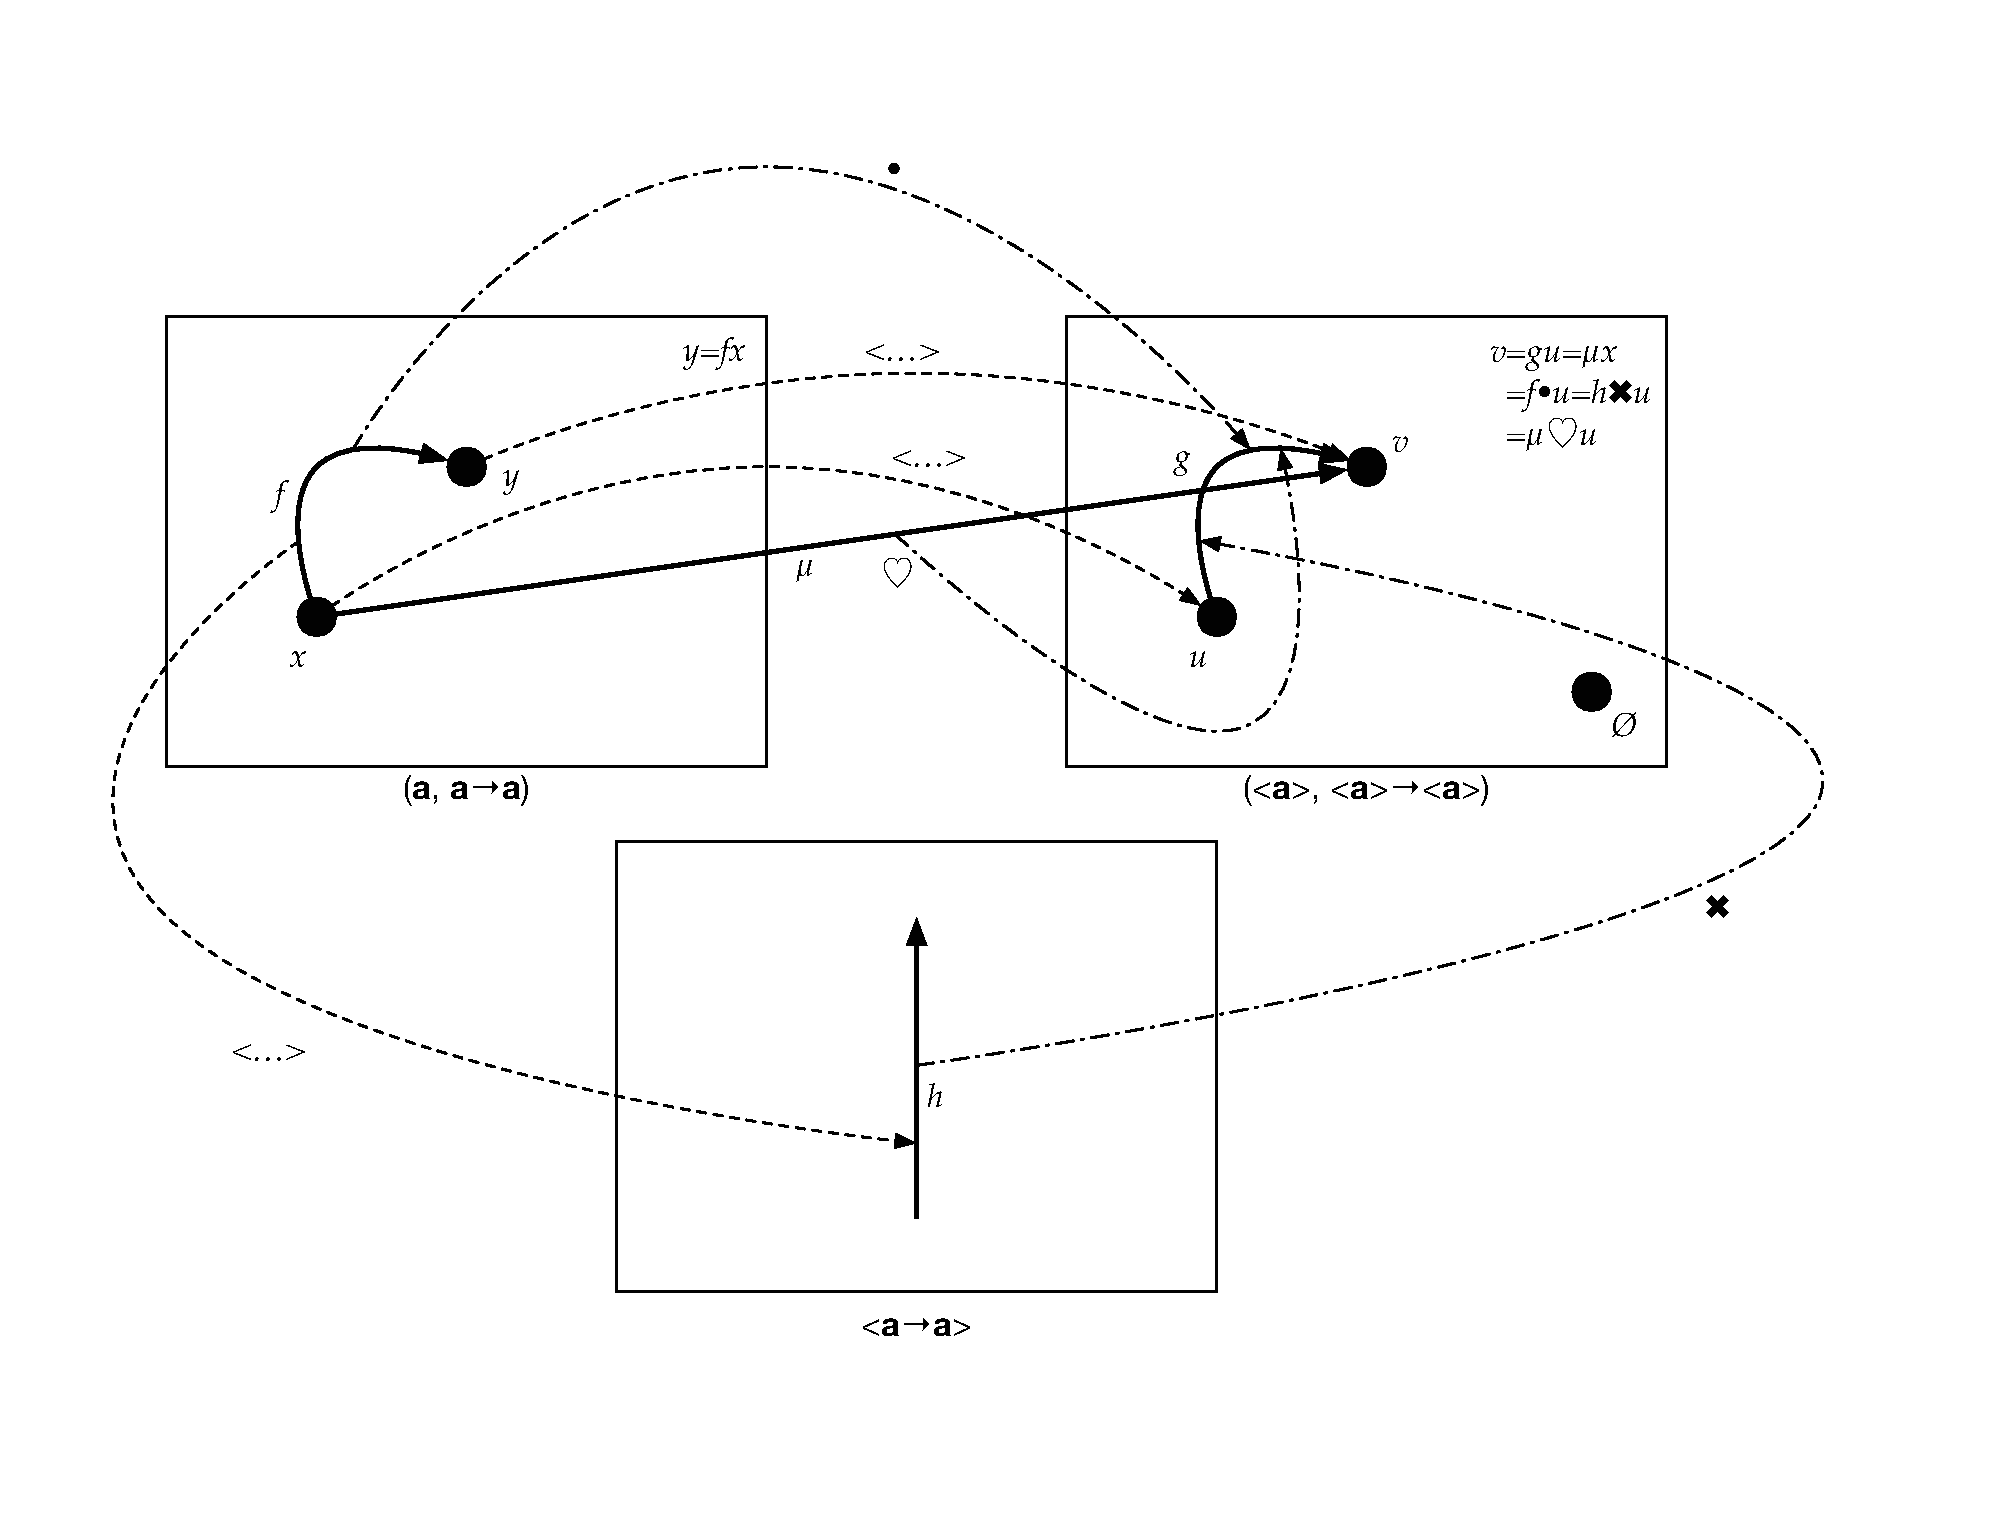
\includegraphics[width=140mm]{fig/functor.eps}
\end{center}
\caption{...}
\label{fig:functor}
\end{figure}


% \section{IOモナド*}

\section{余計な話:モナドプラス}

\chapter{IO}

\chapter{代数的構造}

\begin{leader}
この章では「代数的構造」を見ていくことにする.代数的構造とは,四則演算のような数に関する基本的な性質を抽象化していくことで,数の背後にある基本的なメカニズムを抽出したものである.代数的構造はあらゆるプログラミング言語に明示的,あるいは非明示的に見られる要素である.
\end{leader}

\section{数}

これから各種の\keyword{代数的構造}を見ていくことにする.代数的構造と言っても,身構える必要はない.それは,我々プログラマが日々接している概念に,共通した名前を与えたにすぎない.

まず最初に,我々にとって一番身近な代数的構造である\keyword{数}を見てみよう.数の代表例は\keyword{実数}であるから,実数を例にとって考えてみよう.実数全体の集合を$\mathSpecialSet{R}$で表すことにする.また任意の実数を$x,y,z$で表すこととする.このことを数学者は$x,y,z\in\mathSpecialSet{R}$と書くが,我々は記号$\in$を別の用途に使いたいので,本書では
\begin{equation}
x,y,z\mathIn\mathSpecialSet{R}
\end{equation}
と表すことにする.

以下に実数の備える代数的性質を列挙する.どれも当たり前のことに見えるが,ひとつひとつ見ていこう.ここで$x,y,z\mathIn\mathSpecialSet{R}$とする.
\begin{description}
\item[実数の性質1. 足し算の全域性] 任意の$x$と任意の$y$の足し算(\keyword{加法})の結果(\keyword{和})$x+y$は$\mathSpecialSet{R}$の元すなわち実数である.演算の結果が同じ集合の元になることを\keyword{全域性}と呼ぶ.
\item[実数の性質2. 足し算の結合性] 任意の$x,y,z$について
\begin{equation}
(x+y)+z=x+(y+z)
\end{equation}
である.これを足し算の\keyword{結合性}(結合律)と呼ぶ.
\item[実数の性質3. 零元(加法単位元)の存在] 特別な実数$0\mathIn\mathSpecialSet{R}$があり
\begin{equation}
0+x=x+0=x
\end{equation}
である.この$0$は足し算の\keyword{単位元}である.\keyword{零元}または\keyword{加法単位元}と呼ぶこともある.単位元が存在することを単位律と呼ぶこともある.
\item[実数の性質4. 負元(加法逆元)の存在] 任意の$x$に対して$-x\mathIn\mathSpecialSet{R}$があり
\begin{equation}
-x+x=0
\end{equation}
である.この$-x$は$x$の足し算の\keyword{逆元}である.\keyword{負元}または\keyword{加法逆元}と呼ぶこともある.逆元が存在することを消約律と呼ぶこともある.
\item[実数の性質5. 足し算の可換性] 任意の$x,y$について
\begin{equation}
x+y=y+x
\end{equation}
である.このことを足し算の\keyword{可換性}(可換律)と呼ぶ.
\item[実数の性質6. 掛け算] 任意の$x$と任意の$y$の掛け算(\keyword{乗法})の結果(\keyword{積})$x*y$は$\mathSpecialSet{R}$の元すなわち実数である.
\item[実数の性質7. 掛け算の結合性] 任意の$x,y,z$について
\begin{equation}
(x*y)*z=x*(y*z)
\end{equation}
である.
\item[実数の性質8. 単位元の存在] 特別な実数$1\mathIn\mathSpecialSet{R}$があり
\begin{equation}
1*x=x*1=x
\end{equation}
である.この$1$を掛け算の単位元または\keyword{乗法単位元}と呼ぶ.
\item[実数の性質9. 逆元の存在] 任意の$x$に対して$x^{-1}\mathIn\mathSpecialSet{R}$があり
\begin{equation}
x^{-1}*x=1
\end{equation}
である.この$x^{-1}$は$x$の掛け算の逆元である.\keyword{乗法逆元}と呼ぶこともある.ただし性質11で述べる通り,加法単位元については逆元がなくても良い.
\item[実数の性質10. 掛け算の可換性] 任意の$x,y$について
\begin{equation}
x*y=y*x
\end{equation}
である.このことを掛け算の可換性と呼ぶ.
\item[実数の性質11. 加法単位元の乗法逆元] 加法単位元に対する掛け算の逆元は存在しなくても良い.(つまり$0^{-1}$のことは考えなくて良い.)
\item[実数の性質12. 分配律] 足し算と掛け算が混在する場合
\begin{equation}
(x+y)*z=(x*z)+(y*z)
\end{equation}
と掛け算を\keyword{分配}する.
\end{description}
以上が実数の代数的性質の全てである.我々がよく使う引き算,割り算は数学上は糖衣構文 (syntax sugar) である.

上述の12個の条件が当てはまる数には,\keyword{有理数}や\keyword{複素数}がある.この12個の性質をまとめて,数学では\keyword{体}と呼ぶ.

体の要素は,集合$\mathSet{K}$,二項演算子$+$,二項演算子$+$の単位元$0$,二項演算子$+$の逆元生成演算子$-$,もう一つの二項演算子$*$,二項演算子$*$の単位元$1$,二項演算子$*$の逆元生成演算子$\mathSomething^{-1}$であるから,体はそれらを列挙して$\mathField{\mathSet{K}}{+}{0}{-}{*}{1}{\mathSomething^{-1}}$と表現する.

体の性質から言えることを一つ紹介しよう.これから
\begin{equation}
z\uparrow n=\underbrace{z*\dotsb*z}_n
\end{equation}
なる二項演算子$\uparrow$(\keyword{クヌースの矢印})を使う.ここに$z$を体$\mathField{\mathSet{K}}{+}{0}{-}{*}{1}{\mathSomething^{-1}}$の$\mathSet{K}$の元,$n$を自然数とした.さて$z\uparrow2$は
\begin{equation}
z\uparrow2=z*z
\end{equation}
であるから,いま$z=x+y$とすると
\begin{align}
z\uparrow2&=z*z\\
&=z*(x+y)\\
&=z*x+z*y\;\text{---分配律}\\
&=(x+y)*x+(x+y)*y\\
&=x*x+y*x+x*y+y*y\;\text{---分配律}\\
&=x\uparrow2+x*y+y*x+y\uparrow2
\end{align}
となり
\begin{equation}
\label{eq:xysq}
(x+y)\uparrow2=x\uparrow2+x*y+y*x+y\uparrow2
\end{equation}
を得る.式\eqref{eq:xysq}は体の性質だけを使って導いた関係なので,実数だけでなく有理数や複素数にもそのまま使える.実際には式\eqref{eq:xysq}は体の性質のうち分配律だけを使っいるので,体以外にも応用が利く式でもある.\footnote{Knuthの矢印は\haskell では演算子\code{\^}として提供されている.}

\begin{table*}
\caption{代表的な代数的構造の性質(1)}
\label{tab:field-and-ring}
\begin{center}
\begin{tabular}{||c||c|c|c|c|c|c||}
\hline
代数的構造&$\mathAnyBinaryOperator_1$&$\mathAnyBinaryOperator_1$の単位元&$\mathAnyBinaryOperator_1$の逆元&$\mathAnyBinaryOperator_2$&$\mathAnyBinaryOperator_2$の単位元&$\mathAnyBinaryOperator_2$の逆元\\
\hline\hline
体&可換&あり&あり&可換&あり&あり\\
環&可換&あり&あり&非可換&あり&なし\\
\hline
\end{tabular}
\end{center}
\end{table*}

\section{群}

体の性質を若干緩めたい場合がある.さもなければ,\keyword{整数},\keyword{正方行列},\keyword{クォータニオン}(四元数),\keyword{論理値},\keyword{ベクトル},ベクトルの\keyword{変換},集合から集合への\keyword{写像}と言った重要な概念が数の概念からこぼれてしまうからである.例えば整数の掛け算の逆元は(単位元の逆元を除いて)整数の中には存在しないし,正則行列やクォータニオンの場合は掛け算が可換ではない.

だいたいどの辺まで制約を緩めたものを数の仲間に入れるかというのは見解の分かれるところでもあるが,体から性質9(掛け算の逆元),性質10(掛け算の可換性),性質11(加法単位元の乗法逆元)を取り除いたものを\keyword{環}と呼び,環の性質を持つものを数の仲間に入れることが一般的である.環の性質を持つものは,体である実数,有理数,複素数に加えて,整数,正方行列,クォータニオン,論理値などがある.

制約を少しずつ緩める代わりに,制約をその構成要素に分解するほうがさらなる応用が利きそうである.体には二つの二項演算子$+$と$*$が登場した.その片方にのみ注目してみたらどうなるだろう.それがこの節で取り上げる\keyword{群}である.

形式的に二項演算子$+$を$\mathAnyBinaryOperator_1$とし,二項演算子$*$を$\mathAnyBinaryOperator_2$として,体と環の性質を並べたものが表\ref{tab:field-and-ring}である.これを見ると,演算子$\mathAnyBinaryOperator$について「可換・単位元あり・逆元あり」の組み合わせが二つペアになったもの(体)か,「可換・単位元あり・逆元あり」の組み合わせと「非可換・単位元あり・逆元なし」の組み合わせがペアになったもの(環)があり,その構成要素は二項演算子$\mathAnyBinaryOperator$について「可換・単位元あり・逆元あり」と「非可換・単位元あり・逆元なし」の2種類であることがわかる.

いま集合$\mathSet{G}$があり,$x,y,z\mathIn\mathSet{G}$であるとし,二項演算子を$\mathAnyBinaryOperator$と書くことにして,体の性質の前半分を書き下してみよう.
\begin{description}
\item[性質1.] 任意の$x$と任意の$y$の演算の結果$x\mathAnyBinaryOperator y$は$\mathSet{G}$の元である.
\item[性質2.] 任意の$x,y,z$について
\begin{equation}
(x\mathAnyBinaryOperator y)\mathAnyBinaryOperator z=x\mathAnyBinaryOperator(y\mathAnyBinaryOperator z)
\end{equation}
である.
\item[性質3.] 特別な元$O\mathIn\mathSet{G}$があり
\begin{equation}
O\mathAnyBinaryOperator x=x\mathAnyBinaryOperator O=x
\end{equation}
である.
\item[性質4.] 任意の$x$に対して$\mathInverse x\mathIn\mathSet{G}$があり
\begin{equation}
\mathInverse x\mathAnyBinaryOperator x=O
\end{equation}
である.
\item[性質5.] 任意の$x,y$について
\begin{equation}
x\mathAnyBinaryOperator y=y\mathAnyBinaryOperator x
\end{equation}
である.
\end{description}
このような性質が満たされる時,組み合わせ$\mathGroup{\mathSet{G}}{\mathAnyBinaryOperator}{O}{\mathInverse}$を\keyword{可換群}または\keyword{加群}と呼ぶ.この可換群が最初の構成要素「可換・単位元あり・逆元あり」の正体である.

例えば$\mathGroup{\mathSpecialSet{R}}{+}{0}{-}$は可換群である.整数全体の集合を$\mathSpecialSet{Z}$とすると$\mathGroup{\mathSpecialSet{Z}}{+}{0}{-}$も可換群である.また,集合$\mathSpecialSet{R}$から$0$だけを取り除いた集合を$\mathSpecialSet{R}\setminus0$とするとき$\mathGroup{\mathSpecialSet{R}\setminus0}{*}{1}{\mathSomething^{-1}}$も可換群である.

可換群は代表的な代数的構造のひとつであり,他にも数学のあちこちに顔を出している.例えば回転角を$t$とする二次元の回転変換を$R_t$として,回転変換$R_t$すべてからなる集合$\mathSet{R}$を考えてみよう.回転の合成を$\bullet$で表すとすると
\begin{equation}
\label{eq:rotation}
R_{t_1}\bullet R_{t_2}=R_{(t_1+t_2)}
\end{equation}
であるから,回転を合成した結果も回転である.また式\eqref{eq:rotation}から
\begin{equation}
R_{t_1}\bullet\left(R_{t_2}\bullet R_{t_3}\right)=\left(R_{t_1}\bullet R_{t_2}\right)\bullet R_{t_3}
\end{equation}
であるから,回転変換は結合性も満たしている.

次にに回転変換に単位元があるかどうか調べてみよう.回転しない変換は\keyword{恒等変換}とも言い,しばしば$I$で表す.何もしない回転変換は$0$度の回転であるから$I=R_0$である.このとき式\eqref{eq:rotation}から
\begin{equation}
I\bullet R_t=R_t\bullet I=R_t
\end{equation}
であるから,$I$は回転変換の単位元であると言える.

最後に回転変換に逆元があるかも調べてみよう.$t$回転の逆は明らかに$-t$であるから
\begin{equation}
R_{-t}\bullet R_t=R_t\bullet R_{-t}=I
\end{equation}
が成り立つ.そこで
\begin{equation}
{R_t}^{-1}=R_{-t}
\end{equation}
として$R_t$の逆元${R_t}^{-1}$を定義することができる.

このように,組み合わせ$\mathGroup{\mathSet{R}}{\bullet}{I}{\mathSomething^{-1}}$も可換群である.(回転$R_t$全体の集合$\mathSet{R}$が群を形成することは,パラメタ$t$が所属する実数全体の集合$\mathSpecialSet{R}$が群を形成することに大いに頼っている.この部分を詳細に調べるとリー群という美しい代数的構造が見つかる.)

回転されるものをベクトルと呼ぶ.ベクトルや回転変換の実装方法はいくつかあり,例えば第1座標値を$u$,第2座標値を$v$としたときにベクトル$\mathVectorVar{p}$を
\begin{equation}
\mathVectorVar{p}=\begin{bmatrix}u\\v\end{bmatrix}
\end{equation}
と表すことにしよう.矢印は変数$p$がベクトルであることを忘れないようにするための飾りである.このとき,回転変換は
\begin{equation}
R_t=\begin{bmatrix}\cos t&-\sin t\\\sin t&\cos t\end{bmatrix}
\end{equation}
と行列で表すことになり,回転後のベクトル$\mathVectorVar{p'}$は
\begin{equation}
\mathVectorVar{p'}=R_t*\mathVectorVar{p}
\end{equation}
となる.ここに演算子$*$は行列の積である.また,この場合変換の合成$\mathCompose$は行列積$*$となる.

他にもベクトルを複素数で表現する方法もある.いま$\mathVectorVar{p}$を
\begin{equation}
\mathVectorVar{p}=u+I v
\end{equation}
と表して,回転変換$R_t$を
\begin{equation}
R_t=\cos t+I\sin t
\end{equation}
とすると,回転後の$\mathVectorVar{p'}$はやはり
\begin{equation}
\mathVectorVar{p'}=R_t*\mathVectorVar{p}
\end{equation}
と書ける.ここに演算子$*$は複素数の積である.また,この場合変換の合成$\mathCompose$も複素数積$*$となる.

任意次元のベクトル全体からなる集合を$\mathSet{V}$として,零ベクトルを$\mathVectorVar{z}$で表すことにしよう.ここでも矢印はベクトルであることを忘れないようにするための飾りである.ベクトル同士の加算を二項演算子$+$で表し,向きを反転させた逆ベクトル作る演算子を$-$とすると,組み合わせ$\mathGroup{\mathSet{V}}{+}{\mathVectorVar{z}}{-}$もまた可換群である.

可換群の性質のうち最初の4項目だけを満たすものを群と呼ぶ.可換群は群の特別な場合である.現代の数学では$x\mathAnyBinaryOperator y\neq y\mathAnyBinaryOperator x$のように演算子の前後を入れ替えると結果が異なるような演算をよく取り扱うので,一般の群は可換群よりもよく取り上げられ,それ故より短い名前が付けられている.

もう一度組み合わせ$\mathGroup{\mathSet{G}}{\mathAnyBinaryOperator}{O}{\mathInverse}$が群である条件を見ておこう.それは
\begin{description}
\item[群の性質1.] 任意の$x$と任意の$y$の演算の結果$x\mathAnyBinaryOperator y$は$\mathSet{G}$の元である.
\item[群の性質2. 結合性] 任意の$x,y,z$について
\begin{equation}
(x\mathAnyBinaryOperator y)\mathAnyBinaryOperator z=x\mathAnyBinaryOperator(y\mathAnyBinaryOperator z)
\end{equation}
である.
\item[群の性質3. 単位元の存在] 特別な元$O\mathIn\mathSet{G}$があり
\begin{equation}
O\mathAnyBinaryOperator x=x\mathAnyBinaryOperator O=x
\end{equation}
である.
\item[群の性質4. 逆元の存在] 任意の$x$に対して$\mathInverse x\mathIn\mathSet{G}$があり
\begin{equation}
\mathInverse x\mathAnyBinaryOperator x=O
\end{equation}
である.
\end{description}
であった.これらの条件を少し緩め,逆元が存在しなくても良い「緩やかな群」を考えてみる.この「緩やかな群」のことを\keyword{単位的半群}または\keyword{モノイド}と呼ぶ.これが構成要素「非可換・単位元あり・逆元なし」の正体である.

\begin{table}
\caption{代表的な代数的構造の性質 (2)}
\label{tab:group-and-monoid}
\begin{center}
\begin{tabular}{||c||c|c|c||}
\hline
代数的構造&$\mathAnyBinaryOperator$&$\mathAnyBinaryOperator$の単位元&$\mathAnyBinaryOperator$の逆元\\
\hline\hline
可換群&可換&あり&あり\\
群&非可換&あり&あり\\
単位的半群&非可換&あり&なし\\
半群&非可換&なし&なし\\
\hline
\end{tabular}
\end{center}
\end{table}

単位的半群の性質は次の三つである.ただし$x,y,z$が集合$\mathSet{M}$の元であるとする.
\begin{description}
\item[単位的半群の性質1.] 任意の$x$と任意の$y$の演算の結果$x\mathAnyBinaryOperator y$は$\mathSet{M}$の元である.
\item[単位的半群の性質2. 結合性] 任意の$x,y,z$について
\begin{equation}
(x\mathAnyBinaryOperator y)\mathAnyBinaryOperator z=x\mathAnyBinaryOperator(y\mathAnyBinaryOperator z)
\end{equation}
である.
\item[単位的半群の性質3. 単位元の存在] 特別な元$O\mathIn\mathSet{M}$があり
\begin{equation}
O\mathAnyBinaryOperator x=x\mathAnyBinaryOperator O=x
\end{equation}
である.
\end{description}
このとき,組み合わせ$\mathMonoid{\mathSet{M}}{\mathAnyBinaryOperator}{O}$が単位的半群である.可換群とこの単位的半群を組み合わせたのが環,可換群二つを組み合わせたのが体であった.

なお,これまで単位元の定義として
\begin{equation}
O\mathAnyBinaryOperator x=x\mathAnyBinaryOperator O=x
\end{equation}
を掲げているが,厳密には単位元は
\begin{equation}
O_\mathLeft\mathAnyBinaryOperator x=x\mathAnyBinaryOperator O_\mathRight=x
\end{equation}
のように,\keyword{左単位元}と\keyword{右単位元}を区別しても良い.

単位的半群の性質からさらに性質3を消したものを\keyword{半群}と呼ぶ.可換群,群,単位的半群,半群を一覧にしたものを表\ref{tab:group-and-monoid}に掲げる.

\section{圏}

これまでは集合の元同士に対する二項演算を考えてきた.集合$\mathSet{M}$が単位的半群であるとき,集合$\mathSet{M}$の元$x,y\mathIn\mathSet{M}$に対して$x\mathAnyBinaryOperator y\mathIn\mathSet{M}$であった.見方を変えると,演算子$\mathAnyBinaryOperator$とは集合$\mathSet{M}$の元2個から出発して,集合$\mathSet{M}$の元1個へとジャンプさせる\keyword{写像}であると言える.これを
\begin{equation}
\mathAnyBinaryOperator\mathIn{}\mathMorph{(\mathSet{M}\mathSetTimes\mathSet{M})}{\mathSet{M}}
\end{equation}
と書く.ここに$\mathSet{X}\mathSetTimes\mathSet{Y}$は集合$\mathSet{X}$と集合$\mathSet{Y}$の\keyword{直積集合}である.直積集合と元の集合はもはや別な集合であることに注意しよう.

写像は$\mathMorph{\mathSet{M}\mathSetTimes\mathSet{M}}{\mathSet{M}}$に限ったもの出はなく,集合$\mathSet{M}$から集合$\mathSet{M}$への写像$\mathAnyUnaryOperator$ただし
\begin{equation}
\mathAnyUnaryOperator\mathIn\mathMorph{\mathSet{M}}{\mathSet{M}}
\end{equation}
があっても良い.実はこれまでにも登場した逆元を作る演算子はまさに$\mathMorph{\mathSet{M}}{\mathSet{M}}$という写像である.

またベクトルには,実数倍や回転といった写像がある.これらは実数のパラメタを一つとるので,ベクトル全体の集合を$\mathSet{V}$,実数全体の集合を$\mathSpecialSet{R}$として,実数のパラメタを$r$としたときに
\begin{equation}
\mathAnyUnaryOperator_r\mathIn{}\mathMorph{(\mathSpecialSet{R}\mathSetTimes\mathSet{V})}{\mathSet{V}}
\end{equation}
と書ける.例えば回転の場合は$\mathAnyUnaryOperator_r=R_r$である.

このようにとある集合(例えば$\mathSet{M}\mathSetTimes\mathSet{M}$や$\mathSpecialSet{R}\mathSetTimes\mathSet{V}$)から異なる別な集合(例えば$\mathSet{M}$や$\mathSet{V}$)へという写像を一般化するとどうなるだろうか.いま,集合$\mathSet{X}$から集合$\mathSet{Y}$への写像$f$があり,集合$\mathSet{Y}$から集合$\mathSet{Z}$への写像$g$があるとする.すなわち
\begin{align}
f&\mathIn\mathMorph{\mathSet{X}}{\mathSet{Y}}\\
g&\mathIn\mathMorph{\mathSet{Y}}{\mathSet{Z}}
\end{align}
があるとする.また写像同士を二項演算子$\mathCompose$で\keyword{合成}できるものとする.例えば$f$と$g$の合成写像は$\mathSet{X}$を出発点に$\mathSet{Y}$を経由して$\mathSet{Z}$へと行くので
\begin{equation}
f\mathCompose g\mathIn\mathMorph{\mathSet{X}}{\mathSet{Z}}
\end{equation}
と書ける.ここで合成演算子は結合性を満たすものとしておこう.

さらに
\begin{equation}
I_\mathSet{X}\mathIn\mathMorph{\mathSet{X}}{\mathSet{X}},\;I_\mathSet{Y}\mathIn\mathMorph{\mathSet{Y}}{\mathSet{Y}},\;I_\mathSet{Z}\mathIn\mathMorph{\mathSet{Z}}{\mathSet{Z}}
\end{equation}
という写像もあるとしよう.ここで
\begin{equation}
I_\mathSet{Y}\mathCompose f=f\mathCompose I_\mathSet{X}
\end{equation}
とすると,写像$I_\mathSet{X}$と写像$I_\mathSet{Y}$はそれぞれ写像の合成演算子$\mathCompose$に対して単位元のように振る舞う.写像$g$については
\begin{equation}
I_\mathSet{Z}\mathCompose g=g\mathCompose I_\mathSet{Y}
\end{equation}
であるとする.このような写像$I_\mathSet{X},I_\mathSet{Y},I_\mathSet{Z}$を\keyword{恒等写像}と呼ぶ.

集合$\mathSet{X}$,集合$\mathSet{Y}$,集合$\mathSet{Z}$の集合$\mathSet{C}=\{\mathSet{X},\mathSet{Y},\mathSet{Z}\}$と,写像$f$と写像$g$の集合$\mathSet{P}=\{f,g\}$と,写像合成演算子$\mathCompose$と,恒等写像の集合$\mathSet{I}$の組み合わせ$\mathCategory{\mathSet{C}}{\mathSet{P}}{\mathCompose}{\mathSet{I}}$を\keyword{圏}と呼ぶ.写像合成演算子$(\mathCompose)$と恒等写像の集合$(\mathSet{I})$は自明であるためしばしば省略され,組み合わせ$\mathCategoryShort{\mathSet{C}}{\mathSet{P}}$を圏とする書き方もよくされる.

圏を考えるとき,変換や写像は全て\keyword{射}と呼ぶ決まりである.

いまある単位的半群$\mathMonoid{\mathSet{M}}{\mathAnyBinaryOperator}{O}$があるとする.集合$\mathSet{C}$を$\mathSet{M}$及び$\mathSet{M}\mathSetTimes\mathSet{M}$を元とする集合すなわち
\begin{equation}
\mathSet{C}=\{\mathSet{M},\mathSet{M}\mathSetTimes\mathSet{M}\}
\end{equation}
とし,集合$\mathSet{P}$を$\mathAnyBinaryOperator$のみを元とする集合すなわち
\begin{equation}
\mathSet{P}=\{\mathAnyBinaryOperator\}
\end{equation}
とすると,組み合わせ$\mathCategoryShort{\mathSet{C}}{\mathSet{P}}$は圏になっている.

\section{余計な話:束*}

A...


\chapter{圏とモナドとプログラミング言語}


\section{クライスリ・トリプル*}

\begin{table*}
\begin{center}
\begin{tabular}{||c||c|c|c|c|c||}
\hline
&Totality&Associativity&Identity&Divisibility&Commutativity\\
\hline\hline
Semicategory&&$\checkmark$&&&\\
Category&&$\checkmark$&$\checkmark$&&\\
Groupoid&&$\checkmark$&$\checkmark$&$\checkmark$&\\
Magma&$\checkmark$&&&&\\
Quasigroup&$\checkmark$&&&$\checkmark$&\\
Loop&$\checkmark$&&$\checkmark$&$\checkmark$&\\
Semigroup&$\checkmark$&$\checkmark$&&&\\
Monoid&$\checkmark$&$\checkmark$&$\checkmark$&&\\
Group&$\checkmark$&$\checkmark$&$\checkmark$&$\checkmark$&\\
Abelian Group&$\checkmark$&$\checkmark$&$\checkmark$&$\checkmark$&$\checkmark$\\
\hline
\end{tabular}
\end{center}
\end{table*}

\begin{table*}
\caption{代数的構造}
\label{tab:algebraicstrcture}
\begin{center}
\begin{tabular}{||c||c|c|c|c|c||}
\hline
&全域性&結合性&単位律&消約律&可換性\\
\hline\hline
半圏(semicategory)&&$\checkmark$&&&\\
圏(category)&&$\checkmark$&$\checkmark$&&\\
亜群(groupoid)&&$\checkmark$&$\checkmark$&$\checkmark$&\\
マグマ(magma)&$\checkmark$&&&&\\
擬群(quasigroup)&$\checkmark$&&&$\checkmark$&\\
ループ(loop)&$\checkmark$&&$\checkmark$&$\checkmark$&\\
半群(semigroup)&$\checkmark$&$\checkmark$&&&\\
モノイド(monoid)&$\checkmark$&$\checkmark$&$\checkmark$&&\\
群(group)&$\checkmark$&$\checkmark$&$\checkmark$&$\checkmark$&\\
可換群(Abelian group)&$\checkmark$&$\checkmark$&$\checkmark$&$\checkmark$&$\checkmark$\\
\hline
\end{tabular}
\end{center}
\end{table*}

% 亜群(groupoid)を中国語では「廣(広)群」と書く.亜群はかつてはマグマの訳語として我が国で用いられていた.
% 擬群のことを準群と呼ぶこともある.この場合ループを擬群と呼ぶこともある.

\section{ラムダ*}

\part{\haskell プログラミング}

\chapter{プログラム}

\begin{leader}
A...
\end{leader}


\section{文字セットとコメント}

\haskell コンパイラを含む多くのコンパイラがUnicode文字セットに対応しているものの,従来からの習慣や英語圏での使いやすさを考慮してか,ASCII文字セットだけでプログラムを書けるようにしているし,またそれを推奨さえしている.

\haskell プログラムもまた,文字定数を除いてはASCII文字セットの範囲で書くことが普通である.そこで我々もその習慣に従うことにしよう.例えば円周率を代入する変数を$\pi$と書きたいところだが,我々は\code{pi}と書く.

数学記号のほとんども,ASCII文字セットの中から記号を組み合わせるか,さもなくば言葉で表現する.例えば\haskell では$\in$の代わりに\code{<-}を使うし,$\wedge$の代わりに\code{and}を使う.

また計算機科学者たちの絶えざる努力にもかかわらず,プログラム中の文字の装飾はこれまでほとんど受け入れられていない.我々は本書で \textrm{f}, \textbf{f}, \textit{f}, $f$ を使い分けてきたが,\haskell プログラム中では全て\code{f}と書く.

以上のような制約にもかかわらず,\haskell プログラムと我々が見えきた「カリー風の」数学記法は本質的に差がない.本書を読み進めてきた読者なら,\haskell プログラムを読むのに苦労はいらないだろう.

なお\haskell では\code{--}から行の終わりまでがコメントとして扱われる.

\section{main関数と一般の関数定義}

\python インタプリタはプログラムを頭から実行していくので,わざわざmain関数を書くことはないが,アプリケーションプログラマにとっての一番の関心事はmain関数の書き方だろう.iOSアプリケーション開発のように,基本的にはmain関数をプログラマが触れないというスタイルもあるが,それでもデバッグの時にはmain関数から辿ることになるので,main関数のありかを知っておくことはいつでも重要だ.

\haskell コンパイラもmain関数をアプリケーションプログラムのエントリポイントとして認識する.というよりも,\haskell プログラムとはmainという一つの関数である.main関数を含む一般の関数はこれまで通り
\begin{equation}
\mathMain=\dots
\end{equation}
のように関数名のあとに等号$(=)$を置いて定義する.

\cxx でmain関数の型がOSの都合で決められているように,\haskell でもmain関数の型はあらかじめ決められている.その型は\code{main :: IO ()}である.


\section{プログラムの本質}

プログラムに与えられた引数やファイルを$x$とし,プログラムの出力を$y$とすると,副作用のないプログラムの本質は
\begin{equation}
y=\mathMain x
\end{equation}
という$\text{main}$関数であり,それを
\begin{equation}
\mathMain=f_1\mathCompose f_2\mathCompose\dots\mathCompose f_n
\end{equation}
と部分関数に分解することがプログラマの能力である.

副作用のない関数を合成するのはわけのないことだ.もし\python ならば
\begin{pythoncode}
% \begin{pythontab}
% \code{y} \pthnOp{=} \code{f}${}_1$(\code{f}${}_2$(\code{x}))
% \end{pythontab}
\begin{verbatim}
y = f1(f2(x))
\end{verbatim}
\end{pythoncode}
のように関数を入れ子にしても良いし,読みづらければ途中経過を一時変数にして
\begin{pythoncode}
% \begin{pythontab}
% \code{y}${}_2$ \pthnOp{=} \code{f}${}_2$(\code{x})\\
% \code{y} \pthnOp{=} \code{f}${}_1$(\pthnId{y}${}_2$)
% \end{pythontab}
\begin{verbatim}
y_2 = f_2(x)
y = f1(y_2)
\end{verbatim}
\end{pythoncode}
としてもよい.副作用のない関数の場合,これが関数合成の規則である.

プログラムが副作用を持つ場合は,文脈を持った変数に入れると見通しが良くなるのであった.文脈を持った変数を$u,v$とするとき,副作用を持つプログラムは
\begin{equation}
v=\mathMain u
\end{equation}
という$\text{main}$関数であり,それを
\begin{equation}
\mathMain=f_1\mathGeneralMap f_2\mathGeneralMap\dots\mathGeneralMap f_n
\end{equation}
と部分関数に分解することがプログラマの能力となる.

\chapter{新しい型の導入}

\section{タプル}

\section{代数型}


% 新しいデータ型を作る http://qiita.com/7shi/items/1ce76bde464b4a55c143


\chapter{IO}

\section{参照透過性とIO}

\section{アクション}

\section{IOモナド}

\begin{haskellcode}
\begin{verbatim}
class
\end{verbatim}
\end{haskellcode}


\chapter{例外}

\section{例外}

\section{do記法}

\chapter{乱数}

\chapter{状態}

\chapter{非決定性}

\chapter{新しい型を作る}

\chapter{木構造}

\chapter{スペースの使い方}

\chapter{継続}

\section{継続とは}




\chapter{Haskellで作る純LISP}

\part{数学の補講}

% \part{\cxx17}
% \chapter{\cxx}

\begin{thebibliography}{99}
\bibitem{haskellplatform} Haskell.org; \texttt{https://www.haskell.org/}, as of 2016.
\bibitem{linux} 大角祐介: 新しいLinuxの教科書; SBクリエイティブ, 2015.
\bibitem{osx} 金谷一朗: 「新しいLinuxの教科書」をMacで実践する; \texttt{http://bit.ly/brew-on-mac}, 2016.
\bibitem{fap} 金谷一朗: ファンクション+アクション=プログラム; 工学社, 2011.
\bibitem{greatgood}Miran Lipovaca: ``Learn You a Haskell for Great Good: A Beginner's Guide''; No Starch Press, 2011.
\bibitem{types} Benjamin C.~Pierce: Types and Programming Languages; The MIT Press, 2002.
\bibitem{patterns} Ryan Lemmer: Haskell Design Patterns; Packt Publishing, 2015.
\bibitem{realworld} Bryan O'Sullivan: ``Real World Haskell: Code You Can Believe In''; O'Reilly Media, 2008.
\bibitem{programming} Graham Hutton: Programming in Haskell; Cambridge University Press; 2007.
\bibitem{functionally} Richard Bird: Thinking Functionally with Haskell; Cambridge University Press, 2014.
\bibitem{gentle} Paul Hudak, John Peterson, Joseph Fasel: A Gentle Guide to Haskell; \texttt{https://www.haskell.org/tutorial/index.html}, 1999.
\end{thebibliography}


\end{document}
